%%%%%%%%%%%%%%%%%%%%%%%%%%%%%%%%%%%%%%%%%%%%%%%%%%%%%%%%%%%%%%%%%%%%%%
%%  disstemplate.tex, to be compiled with latex.		     %
%%  08 April 2002	Version 4				     %
%%%%%%%%%%%%%%%%%%%%%%%%%%%%%%%%%%%%%%%%%%%%%%%%%%%%%%%%%%%%%%%%%%%%%%
%%								     %
%%  Writing a Doctoral Dissertation with LaTeX at		     %
%%	the University of Texas at Austin			     %
%%								     %
%%  (Modify this ``template'' for your own dissertation.)	     %
%%								     %
%%%%%%%%%%%%%%%%%%%%%%%%%%%%%%%%%%%%%%%%%%%%%%%%%%%%%%%%%%%%%%%%%%%%%%


\documentclass[12pt]{report}	% The documentclass must be ``report''.

\usepackage{utdiss2}  		% Dissertation package style file.


%%%%%%%%%%%%%%%%%%%%%%%%%%%%%%%%%%%%%%%%%%%%%%%%%%%%%%%%%%%%%%%%%%%%%%
% Optional packages used for this sample dissertation. If you don't  %
% need a capability in your dissertation, feel free to comment out   %
% the package usage command.					     %
%%%%%%%%%%%%%%%%%%%%%%%%%%%%%%%%%%%%%%%%%%%%%%%%%%%%%%%%%%%%%%%%%%%%%%

\usepackage{amsmath,amsthm,amsfonts,amscd, amssymb} 
				% Some packages to write mathematics.
\usepackage{eucal} 	 	% Euler fonts
\usepackage{verbatim}      	% Allows quoting source with commands.
\usepackage{makeidx}       	% Package to make an index.
\usepackage{psfig}         	% Allows inclusion of eps files.
\usepackage{epsfig}         	% Allows inclusion of eps files.
%\usepackage{citesort}         	% 
\usepackage{url}		% Allows good typesetting of web URLs.
%\usepackage{draftcopy}		% Uncomment this line to have the
				% word, "DRAFT," as a background
				% "watermark" on all of the pages of
				% of your draft versions. When ready
				% to generate your final copy, re-comment
				% it out with a percent sign to remove
				% the word draft before you re-run
				% Makediss for the last time.

%The Rest of these are packages that I need for my thesis.
\usepackage{hyperref}
\usepackage{amsfonts}
\usepackage{graphicx}
\usepackage[english]{babel}
%\usepackage[
%backend=biber,
%style=alphabetic,
%sorting=ynt
%]{biblatex}
\usepackage{tikz}
\usepackage{algorithm}
\usepackage{algorithmicx}
\usepackage[noend]{algpseudocode}
\usepackage{geometry}
\usepackage{marginnote}
\usepackage{csquotes}

%\addbibresource{bibliography.bib}



\author{Matthew Alexander Denend}  	% Required

%Used email address as I STRONGLY preferred this as opposed 
%to physical address. 
\address{mad4672@cs.utexas.edu}  % Required

\title{Challenging Variants of the Collatz Conjecture}
                                                    % Required

%%%%%%%%%%%%%%%%%%%%%%%%%%%%%%%%%%%%%%%%%%%%%%%%%%%%%%%%%%%%%%%%%%%%%%
% NOTICE: The total number of supervisors and other members %%%%%%%%%%
%%%%%%%%%%%%%%% MUST be seven (7) or less! If you put in more, %%%%%%%
%%%%%%%%%%%%%%% they are put on the page after the Committee %%%%%%%%%
%%%%%%%%%%%%%%% Certification of Approved Version page. %%%%%%%%%%%%%%
%%%%%%%%%%%%%%%%%%%%%%%%%%%%%%%%%%%%%%%%%%%%%%%%%%%%%%%%%%%%%%%%%%%%%%

%%%%%%%%%%%%%%%%%%%%%%%%%%%%%%%%%%%%%%%%%%%%%%%%%%%%%%%%%%%%%%%%%%%%%%
%
% Enter names of the supervisor and co-supervisor(s), if any,
% of your dissertation committee. Put one name per line with
% the name in square brackets. The name on the last line, however,
% must be in curly braces.
%
% If you have only one supervisor, the entry below will read:
%
%	\supervisor
%		{Supervisor's Name}
%
% NOTE: Maximum three supervisors. Minimum one supervisor.
% NOTE: The Office of Graduate Studies will accept only two supervisors!
% 
%
\supervisor
	[Scott Aaronson]
	{Marijn Heule}

%%%%%%%%%%%%%%%%%%%%%%%%%%%%%%%%%%%%%%%%%%%%%%%%%%%%%%%%%%%%%%%%%%%%%%
%
% Enter names of the other (non-supervisor) members(s) of your
% dissertation committee. Put one name per line with the name
% in square brackets. The name on the last line, however, must
% be in curly braces.
%
% NOTE: Maximum six other members. Minimum zero other members.
% NOTE: The Office of Graduate Studies may restrict you to a total
%	of six committee members.
%
%
%\committeemembers
%	[Erwin Schr\"odinger]
%	[Albert Einstein]
%	[Charles Townes]
%	{Arthur Schawlow}

%%%%%%%%%%%%%%%%%%%%%%%%%%%%%%%%%%%%%%%%%%%%%%%%%%%%%%%%%%%%%%%%%%%%%%

\previousdegrees{B.S.}
     % The abbreviated form of your previous degree(s).
     % E.g., \previousdegrees{B.S., MBA}.
     %
     % The default value is `B.S., M.S.'

%\graduationmonth{...}      
     % Graduation month, either May, August, or December, in the form
     % as `\graduationmonth{May}'. Do not abbreviate.
     %
     % The default value (either May, August, or December) is guessed
     % according to the time of running LaTeX.

%\graduationyear{...}   
     % Graduation year, in the form as `\graduationyear{2001}'.
     % Use a 4 digit (not a 2 digit) number.
     %
     % The default value is guessed according to the time of 
     % running LaTeX.

%\typist{...}       
     % The name(s) of typist(s), put `the author' if you do it yourself.
     % E.g., `\typist{Maryann Hersey and the author}'.
     %
     % The default value is `the author'.


%%%%%%%%%%%%%%%%%%%%%%%%%%%%%%%%%%%%%%%%%%%%%%%%%%%%%%%%%%%%%%%%%%%%%%
% Commands for master's theses and reports.			     %
%%%%%%%%%%%%%%%%%%%%%%%%%%%%%%%%%%%%%%%%%%%%%%%%%%%%%%%%%%%%%%%%%%%%%%
%
% If the degree you're seeking is NOT Doctor of Philosophy, uncomment
% (remove the % in front of) the following two command lines (the ones
% that have the \ as their second character).
%
\degree{MASTER OF SCIENCE}
\degreeabbr{M.S.}

% Uncomment the line below that corresponds to the type of master's
% document you are writing.
%
%\masterreport
\masterthesis


%%%%%%%%%%%%%%%%%%%%%%%%%%%%%%%%%%%%%%%%%%%%%%%%%%%%%%%%%%%%%%%%%%%%%%
% Some optional commands to change the document's defaults.	     %
%%%%%%%%%%%%%%%%%%%%%%%%%%%%%%%%%%%%%%%%%%%%%%%%%%%%%%%%%%%%%%%%%%%%%%
%
%\singlespacing
%\oneandonehalfspacing

%\singlespacequote
\oneandonehalfspacequote

\topmargin 0.125in	% Adjust this value if the PostScript file output
			% of your dissertation has incorrect top and 
			% bottom margins. Print a copy of at least one
			% full page of your dissertation (not the first
			% page of a chapter) and measure the top and
			% bottom margins with a ruler. You must have
			% a top margin of 1.5" and a bottom margin of
			% at least 1.25". The page numbers must be at
			% least 1.00" from the bottom of the page.
			% If the margins are not correct, adjust this
			% value accordingly and re-compile and print again.
			%
			% The default value is 0.125"

		% If you want to adjust other margins, they are in the
		% utdiss2-nn.sty file near the top. If you are using
		% the shell script Makediss on a Unix/Linux system, make
		% your changes in the utdiss2-nn.sty file instead of
		% utdiss2.sty because Makediss will overwrite any changes
		% made to utdiss2.sty.

%%%%%%%%%%%%%%%%%%%%%%%%%%%%%%%%%%%%%%%%%%%%%%%%%%%%%%%%%%%%%%%%%%%%%%
% Some optional commands to be tested.				     %
%%%%%%%%%%%%%%%%%%%%%%%%%%%%%%%%%%%%%%%%%%%%%%%%%%%%%%%%%%%%%%%%%%%%%%

% If there are 10 or more sections, 10 or more subsections for a section,
% etc., you need to make an adjustment to the Table of Contents with the
% command \longtocentry.
%
%\longtocentry 



%%%%%%%%%%%%%%%%%%%%%%%%%%%%%%%%%%%%%%%%%%%%%%%%%%%%%%%%%%%%%%%%%%%%%%
%	Some math support.					     %
%%%%%%%%%%%%%%%%%%%%%%%%%%%%%%%%%%%%%%%%%%%%%%%%%%%%%%%%%%%%%%%%%%%%%%
%I USED MY OWN HERE.
%
%	Theorem environments (these need the amsthm package)
%
%% \theoremstyle{plain} %% This is the default
\newtheorem{theorem}{Theorem}[section]
\newtheorem{corollary}{Corollary}[theorem]
\newtheorem{lemma}[theorem]{Lemma}

\theoremstyle{definition}
\newtheorem{definition}{Definition}[section]
\newtheorem{question}{Question}[section]

\newcommand{\Mod}[1]{\ (\mathrm{mod}\ #1)}
\newcommand{\Col}[1]{\mathrm{Col}(#1)}
\newcommand{\ColMod}[3]{\mathrm{Col}_{\text{mod}}(#1,#2,#3)}
%\newtheorem{thm}{Theorem}[section]
%\newtheorem{cor}[thm]{Corollary}
%\newtheorem{lem}[thm]{Lemma}
%\newtheorem{prop}[thm]{Proposition}
%\newtheorem{ax}{Axiom}

%\theoremstyle{definition}
%\newtheorem{defn}{Definition}[section]

%\theoremstyle{remark}
%\newtheorem{rem}{Remark}[section]
%\newtheorem*{notation}{Notation}

%\numberwithin{equation}{section}


%%%%%%%%%%%%%%%%%%%%%%%%%%%%%%%%%%%%%%%%%%%%%%%%%%%%%%%%%%%%%%%%%%%%%%
%	Macros.							     %
%%%%%%%%%%%%%%%%%%%%%%%%%%%%%%%%%%%%%%%%%%%%%%%%%%%%%%%%%%%%%%%%%%%%%%
%
%	Here some macros that are needed in this document:


\newcommand{\latexe}{{\LaTeX\kern.125em2%
                      \lower.5ex\hbox{$\varepsilon$}}}

\newcommand{\amslatex}{\AmS-\LaTeX{}}

\chardef\bslash=`\\	% \bslash makes a backslash (in tt fonts)
			%	p. 424, TeXbook

\newcommand{\cn}[1]{\texttt{\bslash #1}}

\makeatletter		% Starts section where @ is considered a letter
			% and thus may be used in commands.
\def\square{\RIfM@\bgroup\else$\bgroup\aftergroup$\fi
  \vcenter{\hrule\hbox{\vrule\@height.6em\kern.6em\vrule}%
                                              \hrule}\egroup}
\makeatother		% Ends sections where @ is considered a letter.
			% Now @ cannot be used in commands.

\makeindex    % Make the index

%%%%%%%%%%%%%%%%%%%%%%%%%%%%%%%%%%%%%%%%%%%%%%%%%%%%%%%%%%%%%%%%%%%%%%
%		The document starts here.			     %
%%%%%%%%%%%%%%%%%%%%%%%%%%%%%%%%%%%%%%%%%%%%%%%%%%%%%%%%%%%%%%%%%%%%%%

\begin{document}

\copyrightpage          % Produces the copyright page.


%
% NOTE: In a doctoral dissertation, the Committee Certification page
%		(with signatures) is BEFORE the Title page.
%	In a masters thesis or report, the Signature page
%		(with signatures) is AFTER the Title page.
%
%	If you are writing a masters thesis or report, you MUST REVERSE
%	the order of the \commcertpage and \titlepage commands below.
%
\commcertpage           % Produces the Committee Certification
			%   of Approved Version page (doctoral)
			%   or Signature page (masters).
			%		20 Mar 2002	cwm

\titlepage              % Produces the title page.



%%%%%%%%%%%%%%%%%%%%%%%%%%%%%%%%%%%%%%%%%%%%%%%%%%%%%%%%%%%%%%%%%%%%%%
% Dedication and/or epigraph are optional, but must occur here.      %
%%%%%%%%%%%%%%%%%%%%%%%%%%%%%%%%%%%%%%%%%%%%%%%%%%%%%%%%%%%%%%%%%%%%%%
%
\begin{dedication}
\index{Dedication@\emph{Dedication}}%
Dedicated to my late mother, who never
let her three battles with cancer stop her from loving her two sons and
her husband.
\end{dedication}


%\begin{acknowledgments}		% Optional
%\index{Acknowledgments@\emph{Acknowledgments}}%
%I wish to thank the multitudes of people who helped me. Time would
%fail me to tell of \ldots
%\end{acknowledgments}


% The abstract is required. Note the use of ``utabstract'' instead of
% ``abstract''! This was necessary to fix a page numbering problem.
% The abstract heading is generated automatically.
% Do NOT use \begin{abstract} ... \end{abstract}.
%
\utabstract
\index{Abstract}%
\indent
This hasn't been written by me yet. Going to do this last.



\tableofcontents   % Table of Contents will be automatically
                   % generated and placed here.

%\listoftables      % List of Tables and List of Figures will be placed
\listoffigures     % here, if applicable.



%%%%%%%%%%%%%%%%%%%%%%%%%%%%%%%%%%%%%%%%%%%%%%%%%%%%%%%%%%%%%%%%%%%%%%
% Actual text starts here.					     %
%%%%%%%%%%%%%%%%%%%%%%%%%%%%%%%%%%%%%%%%%%%%%%%%%%%%%%%%%%%%%%%%%%%%%%
%
% Including external files for each chapter makes this document simpler,
% makes each chapter simpler, and allows for generating test documents
% with as few as zero chapters (by commenting out the include statements).
% This allows quicker processing by the Makediss command file in case you
% are not working on a specific, long and slow to compile chapter. You
% can even change the chapter order by merely interchanging the order
% of the include statements (something I found helpful in my own
% dissertation).
%
\chapter{Introduction} \label{sec:introduction}
%Introduction: First sentence: Computers have been very powerful applications for many things, but they don't work for seemingingly simple problems.

%Second sentence: Does  there  exist  a  program  that  can  determine  if  an  arbitrary  program  with arbitrary input will terminate? 

%Will a given program on any input always terminate? Be careful here.

%Turing  proved  that  the  halting  problem  is  undecidable,  because: replace because with in other words, this means that ... make it less formal. 

%As a given problem for all inputs. Make sure this is clear, and resend him another copy of this first paragraph in the near future.

%Algorithm 1 is Classical, 4 is generalization throughout the thesis.  Delete Algorithm 2, and 3 and move Algorithm 4 from section 2 to section 1, use that here.

%Algorithm 1: Collatz Conjecture Recursion. Algorithm 4: A generalization of the Collatz Conjecture Recursion. The Collatz Conjecture halts for some variants of alg. 4. Call Alg 3/4 subscript _{\text{mod}}. Text for names, italic for variables.

%Since  the  Collatz  Conjecture  seems  to  be  quite  difficult  to  prove: replace with Since  the  Collatz  Conjecture  has been challenging to prove, instead o

%This thesis also follows an attempt that Heule and Aaronson have devised to attemptto solve the Collatz Conjecture with computers: replace first attempt with an approach

% At a high level, it involves taking a completely reworked formulation: replace with reformulation.
%HERE IS NEW
Computers have been successfully applied to many complex problems, such as those in finance, healthcare, and the Internet. However, computers still struggle with seemingly simple problems. Consider whether a given program on arbitrary input will always terminate. One can easily show that certain programs will always halt. For example, a program that only prints ``Hello World!'' then exits will always terminate. Nevertheless, there exist simple programs that are much harder to determine if they always terminate. Algorithm~\ref{alg:ColR} is such an example. Will this program always return 1 for any positive integer $N$, causing it to
halt? This problem is a reformulation of the Collatz Conjecture. \par
\begin{algorithm} 
\caption{The Collatz Conjecture Sequence, $\Col{N}$}
\label{alg:ColR} 
\begin{algorithmic}[1]
    \If{$N \leq 1$} \Return $N$ 
    \EndIf
    \If {$N \equiv 0 \Mod{2}$} \Return $\Col{N/2}$
    \EndIf
    \State \Return $\Col{3N + 1}$ 
\end{algorithmic}
\end{algorithm}
We know from Turing that no program exists to determine if an arbitrary program with arbitrary input can halt~\cite{Turing1936}, but that does not exclude the possibility of a program that determines if specifically Algorithm~\ref{alg:ColR} halts. However, no program has been found to show that all inputs for Algorithm~\ref{alg:ColR} will halt, even though this problem can be explained to an elementary grade student. Many approaches have been tried since 1963~\cite{2003mathLagrais}~\cite{2006mathLagrias}. Further, empirical evidence suggests that the Collatz Conjecture is true: according to a website maintained by Eric Roosendahl~\cite{EricRoose}, all numbers up to $87 \cdot 2^{60}$, or about $10^{20}$, have been tried as $N$ in Algorithm~\ref{alg:ColR}, and have converged to 1. \par
Since the Collatz Conjecture has been challenging to prove, we propose another supposedly simpler variant of it. Can we prove that the code in Algorithm \ref{alg:ColSP}, where $A = \{1\}$, and $b = 8$ ($\ColMod{N}{\{1\}}{8}$ is shorthand for this problem), always terminates for any input number? Even though this program seems to be easier, we do not have a program showing this variant always terminates either! \par
\begin{algorithm} 
\caption{A Collatz Conjecture Variant $\ColMod{N}{A}{b}$}
\label{alg:ColSP} 
\begin{algorithmic}[1]
    \If{$(N \leq 1) \vee (N \equiv a_1  \Mod{b}) \vee \ldots \vee (N \equiv a_s \Mod{b})$ } \Return $N$
    \EndIf
    \If {$N \equiv 0 \Mod{2}$} \Return $\ColMod{N/2}{A}{b}$
    \EndIf
    \State \Return $\ColMod{3N+1}{A}{b}$ 
\end{algorithmic}
\end{algorithm}
One of the goals of this Thesis is to try and determine how hard certain variants of the Collatz Conjecture are to solve. A contribution of this thesis is that it uses empirical data to try and find trends of hardness for difficult variants, and compare these trends to the hardness of solving the whole Collatz Conjecture. This thesis also follows an approach that Heule and Aaronson have devised to attempt to craft a program to determine if Algorithm~\ref{alg:ColR} always halts~\cite{HeuleAaronson}. At a high level, it involves taking a completely reworked formulation of Algorithm~\ref{alg:ColR} and using known techniques that, if certain conditions are met, the reworked formulation can be shown to terminate for any input. The formulation requires SAT solvers, string rewrite systems, and a technique called matrix interpretation, all topics which will be covered briefly in this paper as background. An investigation on the difficulty of solving Algorithm~\ref{alg:ColSP} for certain values of $A$ and $b$ using a rewrite system that represents the Collatz Conjecture instead of algebra is another contribution by this thesis.\par
The rest of this thesis is outlined as follows: Chapter~\ref{sec:defns} introduces definitions that will be used throughout the paper. Chapter~\ref{sec:alttercdns} defines several Collatz Conjecture variants, including both solvable ones and unsolved ones, including $\ColMod{N}{\{1\}}{8})$. Chapter~\ref{sec:subhrdnspred} analyzes the difficulty of these variants using algebra. Chapter~\ref{sec:SRSandSAT} provides background on String Rewrite Systems, and how SAT solvers can be used to prove termination of them. Chapter~\ref{sec:CollatzSRS} talks about Aaronson's rewrite system that Heule tried to use with matrix interpretation and SAT solving to prove, and chapter~\ref{sec:provingCollatzresults} presents the results of this approach. Finally, chapter~\ref{sec:hardnessrewriterules} investigates hardness of solving the same variants covered in chapter~\ref{sec:subhrdnspred}, but derived from Aaronson's rewrite system instead.
 %From here, link towards the many approaches that are documented by Lagrias over most of the last 50 years. I don't think the Halting problem is relevant in the introduction anymore, so don't force it.
%At this point, mention the variant.


%BELOW IS OLD.
%Computers, while ubiquitous in everyday life, are not all-powerful. Consider this question, for instance: \textit{Does there exist a program that can determine if an arbitrary program with arbitrary input will terminate?} This is called the halting problem, and Turing in 1936 found that no program can determine if arbitrary code with arbitrary input can exist.~\cite{Turing1936}. More formally, Turing proved that the halting problem is undecidable, because if we turn the halting problem into a decision problem (a yes/no question), we cannot decide the answer.\par
%The halting problem not only had an impact on computer science, but on mathematics as well. An example is the unsolved Collatz Conjecture. The conjecture states that all positive numbers that follow the sequence depicted in Algorithm \ref{alg:ColR} will eventually reach 1. (An iterative version is provided by Algorithm \ref{alg:ColI}).
%\begin{algorithm} 
%\caption{The Collatz Conjecture Sequence, $Col(N)$ (Recursive)}
%\label{alg:ColR} 
%\begin{algorithmic}[1]
%    \If{$N \leq 1$} \Return $N$ 
%    \EndIf
%    \If {$N \equiv 0 \Mod{2}$} \Return $Col(N/2)$
%    \EndIf
%    \State \Return $Col(3N + 1)$ 
%\end{algorithmic}
%\end{algorithm}
%\begin{algorithm} 
%\caption{The Collatz Conjecture Sequence, $Col(N)$ (Iterative)}
%\label{alg:ColI} 
%\begin{algorithmic}[1]
%    \While{$N > 1$} 
%    \If {$N \equiv 0 \Mod{2}$} $N = N/2$
%        \Else \text{ $N = 3N + 1)$}
%        \EndIf
%    \EndWhile
%\end{algorithmic}
%\end{algorithm}

%Algorithm 1 belongs to a class of undecidable problems, as was shown by Conway in 1972~\cite{Conway72} in a paper showing that a generalization of all problems like the Collatz Conjecture be reduced to the halting problem.\footnote{For more detail, see~\cite{2003mathLagrais}, p. 19.}\par
%While the Collatz Conjecture belongs to a class of undecidable problems, this does not mean that the Collatz Conjecture itself is unprovable. However, it seems quite challenging: many approaches have been tried. Lagrias compiled two comprehensive surveys which encapsulate several approaches from 1963-2009~\cite{2003mathLagrais}~\cite{2006mathLagrias}. Further, according to a website maintained by Roosendaal~\cite{EricRoose}, numbers up to $87 \cdot 2^{60}$, or about $10^{20}$, have been tried as $N$ in Algorithm~\ref{alg:ColI}, and all have converged to 1. This further fuels the search for a proof or a counterexample to the Collatz Conjecture. \par
%Since the Collatz Conjecture seems to be quite difficult to prove, we propose another supposedly simpler question. Can we prove that the code in Algorithm \ref{alg:ColM} always terminates for any input number? Even though this seems easier to prove, we do not have a solution for it either! 
%\begin{algorithm} 
%\caption{A Collatz Conjecture Subproblem, $Col_{sub}(N,1,8)$}
%\label{alg:ColM} 
%\begin{algorithmic}[1]
%    \If{$(N \leq 1) \vee (N \equiv 1 \Mod{8})$ } \Return $N$
%    \EndIf
%    \If {$N \equiv 0 \Mod{2}$} \Return $Col_{sub}(N/2,1,8)$
%    \EndIf
%    \State \Return $Col_{sub}(3N + 1,1,8)$ 
%\end{algorithmic}
%\end{algorithm}
%One of the goals of this Thesis is to try and determine how hard this subproblem, and other related subproblems, are to solve. One contribution of this thesis is that it used empirical data to try and find trends of hardness for these subproblems, and compare this to the hardness of solving the whole Collatz Conjecture. \par
%This thesis also follows an attempt that Heule and Aaronson have devised to attempt to solve the Collatz Conjecture with computers~\cite{HeuleAaronson}. At a high level, it involves taking a completely reworked formulation of Algorithm \ref{alg:ColR} and using known techniques that, if certain conditions are met, the reworked formulation can be shown to terminate for any input. The formulation requires SAT solvers, string rewrite systems, and a technique called matrix interpretation, all topics which will be covered in this paper as background. An investigation on the difficulty of solving Algorithm \ref{alg:ColM} and related subproblems using the rewrite system instead of algebra is another contribution by this thesis.\par
%The rest of this paper is outlined as follows: Section~\ref{sec:defns} introduces definitions that will be used throughout the paper. Section~\ref{sec:alttercdns} defines several Collatz Conjecture subproblems, including the one based on Algorithm \ref{alg:ColM}, while section~\ref{sec:subhrdnspred} analyzes the difficulty of these subproblems, algebraically. Section~\ref{sec:SATsolving} provides background on SAT solving. Section~\ref{sec:SRSandSAT} provides background on String Rewrite System, and how SAT solvers can be used to prove termination of them. Section~\ref{sec:CollatzSRS} talks about Aaronson's rewrite system that Heule tried to use with matrix interpretation and SAT solving to prove, and section~\ref{sec:provingCollatzresults} presents the results of this approach. Finally, section~\ref{sec:hardnessrewriterules} investigates hardness of solving the same subproblems covered in section~\ref{sec:subhrdnspred}, but derived from Aaronson's rewrite system instead.


\chapter{Definitions} \label{sec:defns}
We will use the following terms throughout the paper to talk about the $3x+1$ problem:
\begin{itemize}
    \item $\boldsymbol{3x+1}$\textbf{ mapping}: A one step application of $Col(N)$ to some input number $N$.
    \item $\boldsymbol{3x+1}$\textbf{ sequence}: Define this as follows: 
    \begin{align*}
        x_0 = x &= \text{ initial input number} \\
        x_{i+1} &= \begin{cases} 
        x_{i}/2 &\text{ if $x_i$ is even} \\
        3 x_{i} + 1 &\text{ if $x_i$ is odd} \\
        \end{cases}
    \end{align*}
    This sequence can continue for arbitrarily large values of $i$, but we are only interested in following the sequence until $x_i$ for some $i$ is 1, as any value after 1 follows the $1 \rightarrow 4 \rightarrow 2 \rightarrow 1$ cycle indefinitely.
    \item \textbf{Collatz Variant:} For the context of this paper, when we say ``Collatz Subproblem,'' we use Algorithm~\ref{alg:ColSP}, which was defined in the introduction. The shorthand for this will be $Col_{sub}(N,A,b)$, where $A = \{a_1 \ldots a_s\}$ is all of the bases that cause termination of the algorithm. Note that for all $a \in A$, $0 \le a < b$, and $A = \emptyset$ is the same as Algorithm~\ref{alg:ColR}.
    \item \textbf{Number of bits:} For an input number $x$, we say that, written in binary, it has $m$ bits.
    \item \textbf{Binary shifts:} We often write numbers in binary in this Thesis and use shift operators used in C and many other programming languages. One difference is that in this paper, we deal with an arbitrary number of bits. We also never deal with negative numbers, so assume all shifts are logical. Here are the shift operators:
    \begin{itemize}
        \item $\boldsymbol{x<<i}$: This operator left shifts the binary representation of the number $x$ over $i$ indices. The lowest $i$ spots vacated by this shift are replaced by 0 bits. In other words, we are performing the operation $x\cdot 2^i$.
        \item $\boldsymbol{x>>i}$: This operator right shifts the binary representation of the number $x$ over $i$ indices. The lowest $i$ spots disappear. In other words, we are performing the operation $\lfloor x / 2^i \rfloor$. Since all shifts in this paper are logical, any bits vacated by the shift are replaced with 0's.
    \end{itemize}
\end{itemize}


\chapter{Alternative Termination Conditions} \label{sec:alttercdns}
 This section explores the problem originally presented in Algorithm~\ref{alg:ColM} and defines several other problems related to it. Before we investigate these open subproblems, we define a graph paradigm that transforms the $3x+1$ problem into directed graphs that depict the flow for all input numbers modulo base $b$, where $b$ is a power of 2. Then using this graph, we can show that some subproblems are provable, whereas others are not.
 %Instead of trying to directly analyze strings from the rewrite system, we can just compute $3x+1$ sequences directly, and convert numbers back and forth to binary, as needed. Using numbers instead of rewrite strings is far less expensive computationally. Furthermore, if we focus our investigation on the least significant bits of these input numbers, we can easily tie the $D$ rewriting rules, or some modifications thereof, to a graph, which allows us to investigate things such as how many times a rewrite rule can be applied before it cannot be applied anymore, but at a far cheaper cost. We can also analyze the necessity for the odd nodes/rules because odd numbers make the Collatz Conjecture harder to solve, since it causes a number to grow. \par
\section{Defining a Collatz base \textit{b} graph} \label{subsec:colgraph}
Define $G_b=(V,E)$ to be a ``Collatz base $b$ graph'', where $b = 2^k$, and $k$ is nonnegative. Choosing a power of 2 for $b$ allows us to easily reason with binary numbers, which is useful for both several proofs in this section and the String Rewrite System that we will discuss starting in section~\ref{sec:CollatzSRS}. $V$ has $b$ vertices in it, where each vertex is labeled a unique integer in the interval $[0, b-1]$. Vertex $v \in V$ corresponds to $v \Mod{b}$. This paper uses the term ``node $v$'' as shorthand to correspond to the number $v$ in $v \Mod{b}$, as opposed to ``vertex'' $v$ which corresponds to the actual vertex of the graph. Let $x_i$ be the $i$\textsuperscript{th} step of the $3x+1$ sequence for input number $x$, and $x_{i+1}$ be the step after. $E = V \times V$ is a set of directed edges, where, for nodes $u, v \in V$, $(u,v) \in E$ if and only if $x_i \equiv u \Mod{b}$ and $x_{i+1} \equiv v \Mod{b}$ for some $x_i$ and $x_{i+1}$. \par

\section{Lemmas that hold for any base \textit{b} Collatz Graph}
This section contains some lemmas that are used throughout this Thesis. First, we start with a lemma about the number of node transitions in any Collatz base $b$ graph $G_b= (V,E)$.
\begin{lemma}
\label{lem:numOutEdges}
Given a Collatz base $b$ graph, for all $v \in V$, if node $v$ is even, then the vertex $v$ has two outgoing edges. Otherwise, if node $v$ is odd, then the vertex $v$ has only one outgoing edge.
\end{lemma}
\begin{proof}
Take a number $x_i$ that corresponds to node $v$. First, let us consider the case where node $v$ is even. When we divide by 2, we perform $x_i >> 1$, having the least significant 0 drop off. The new bit at index $k-1$ can be either a 0 or a 1, allowing for two options for even nodes. \par
Now, take $x_i$ that corresponds to a node $v$ that is odd. Multiplying $x_i$ by 3 and adding 1 will make the binary string grow at least one bit longer (since $3\cdot x_i = x_i << 1 + x_i$), giving us only one option for the least significant $k$ bits, meaning $x_{i+1}$ can only correspond to one node $w \in V$, and only one such outgoing edge from $v$ exists.
\end{proof}
Now, we have a couple of important properties about cycles that exist in any Collatz base $b$ graph, and the fact that these cycles cannot continue indefinitely. First, we introduce the ``0 cycle'' Lemma.
\begin{lemma}
\label{lem:zeroCycle}
For any Collatz base $b$ graph (where $b$ is a positive power of 2), a self-loop occurs on a 0 node. This cycle cannot continue indefinitely.
\end{lemma}
\begin{proof}
Assume we have an input number $N$ such that $N \equiv 0 \Mod{b}$. This means that the $k$ least significant bits are all 0. Apply the $3x+1$ mapping once to this string. We remove a 0 from the end, since we divide the input number by 2. We now look at the new number $N/2$ and the $k$ least significant bits. The $k-1$ least significant bits are all 0. But what is the value of the bit in the most significant of the $k$ bits? If it is a 0, then our new number $N/2 \equiv 0 \Mod{b}$, and we have a self-loop. \par
To show that the self loop cannot continue indefinitely: every time we follow the self-loop, remove a 0. Since we also know that $N > 1$ in order for the algorithm to continue running, we also know that at least one binary digit is a 1. So as we continue cutting off 0's, we eventually reach a point where the least $k$ significant bits are $1000\ldots 0$, meaning we transition to node $b/2$ instead, ending the cycle.
\end{proof}
Now, we introduce another important lemma about cycles: the fact that we will always have a cycle between nodes $b-2$ and $b-1$. We call this the ``1 Consumption'' Lemma.
\begin{lemma}
\label{lem:oneConsumption}
 For any Collatz base $b$ graph, a cycle between exists between nodes $b-2$ and $b-1$. This cycle cannot continue indefinitely.
\end{lemma}
\begin{proof}
In this proof, we will show first that a $b-1 \rightarrow b-2 \rightarrow b-1$ cycle exists, and second, that this cycle cannot continue indefinitely; more precisely, that some number congruent modulo to $b-2 \Mod{b}$, after division by 2, actually becomes $b/2-1 \Mod{b}$ instead. We will do so using long multiplication in binary, adding the 1 in as well for shorthand. \par
Let $x$ be a arbitrary number congruent modulo to $b-1 \Mod{b}$. We want to express $x$ in binary, so let $x$ have $m$ bits. We know that since $x$ is congruent modulo to $b-1 \Mod{b}$, all bits from indices 0 to $k-1$ are 1. Let $x_j$ denote the $j$\textsuperscript{th} bit of $x$, $k \leq j \leq m$. These indices correspond to unknown bits. Let $1_{+1}$ correspond to the adding of 1 after multiplying by 3, which is added to the 0\textsuperscript{th} index of $x$. Let $c_j$ denote the unknown carry for the $j$\textsuperscript{th} index of bits being added. Let $y$ be the result after $3x+1$ is computed, and let the $j$\textsuperscript{th} index of $y$ be the same index as $x$. The multiplication is referenced in Table~\ref{tab:mul}. \par
\begin{figure}
\begin{tabular}{*{16}c}%{c*{15}{@{\,}c}}
 & & $ x_{n}$  & $ x_{n-1}$  & \ldots & $ x_{j+1}$  & $ x_{j}$  & \ldots & $ x_{k+1}$  & $ x_{k}$  & 1 & 1 & \ldots & 1 & 1 & 1 \\
$\times$ & & & & & & & & & & & & & & 1 & 1 \\
\hline
\tiny ${\scriptscriptstyle c_{n+2}}$ & ${\scriptscriptstyle c_{n+1}}$ & ${\scriptscriptstyle c_{n}}$ & ${\scriptscriptstyle c_{n-1}}$ & & ${\scriptscriptstyle c_{j+1}}$ & ${\scriptscriptstyle c_{j}}$ & & ${\scriptscriptstyle c_{k+1}}$ & \tiny 1 & \tiny 1 &  \tiny 1 & &  \tiny 1 & \tiny 1 & \\
  & & $ x_{n}$  & $ x_{n-1}$  & \ldots & $ x_{j+1}$  & $ x_{j}$  & \ldots & $ x_{k+1}$  & $ x_{k}$  & 1 & 1 & \ldots & 1 & 1 & 1 \\
  + & $ x_{n}$  & $ x_{n-1}$  & $ x_{n-2}$  & \ldots & $ x_{j}$  & $ x_{j-1}$  & \ldots & $ x_{k}$  & 1 & 1 & 1 & \ldots & 1 & 1 & $1_{+1}$  \\
  \hline
  $ y_{n+2}$  & $ y_{n+1}$  & $ y_{n}$  & $ y_{n-1}$  & \ldots & $ y_{j+1}$  & $ y_{j}$  & \ldots & $ y_{k+1}$  & $ y_{k}$  & 1 & 1 & \ldots & 1 & 1 & 0 
\end{tabular}
\caption{The long multiplication corresponding to $3x + 1$. Note how, in the addition step, the $1_{+1}$ is in place of a zero, and the addition is just $x + x << 1 + 1$, where $<<$ is the left shift operator.}
\label{fig:mul}
\end{figure}
Observe that, in binary, multiplication of a binary number $x$ by 3 is just $x + 2x = x + x << 1$. In the multiplication we show in Figure~\ref{fig:mul}, we replace the extra 0 vacated by $x << 1$ with the addition of 1, $1_+1$, allowing us to perform $3x+1$ with just one addition instead of two. \par
Observe that all bits in the resulting binary number $y$ from indices 0 to $k-1$ are 1, except for index 0, which is 0. This is because all bits of $y$, save index 0, are computed by adding $1+1$ and carrying over the 1 from the previous addition. As a result, $y$ is congruent modulo to $b-2 \Mod{b}$, meaning an edge from node $b-1 \Mod{b}$ to node $b-2 \Mod{b}$ exists in our graph.\par
When we divide $y$ by 2, we just perform $y >> 1$. Hence, bit $y_k$ is now in position $k-1$. If $y_k$ is 1, our number is now congruent modulo to $b-1 \Mod{b}$. This means an edge also exists from node $b-2 \Mod{b}$ to node $b-1 \Mod{b}$, proving the existence of the cycle. \par
Now we show that this $b-2 \rightarrow b-1 \rightarrow b-2$ cycle will always eventually terminate. This happens when, after dividing a number congruent modulo to $b-2 \Mod{b}$ by 2, bit $y_{k-1}$ is 0. So we need to show this eventually occurs for any arbitrary $x$. There are two cases for this:
\begin{enumerate}
    \item Some bit in $x$ is 0. Let $x_j$ be the least significant bit of $x$ that is 0 (all bits which have indices lower than $j$ are 1). Look back at Figure~\ref{fig:mul}, and replace $x_j = 0$, and have all bits at indices less than $j$ be 1. After taking the $3x+1$ step, all indices of $y$ between 1 and $j-1$ will be 1, as each time, we add $1 + 1$ and carry over a 1. However, when we get to index $i$, we add $1 + 0$ plus a carry of 1, making bit $y_j = 0$. Since after we divide by 2 we right shift all bits one index, bit $y_j$ now moves to index $j-1$. We repeat this process a total of $j-k+1$ steps. After this, the 0 bit will be in position $y_{k-1}$, making $y$ congruent modulo to $b/2 - 1 \Mod{b}$ instead, breaking the cycle.
    \item No bit in $x$ is 0. In this case, again looking at Figure~\ref{fig:mul}, all bits in $y$ from indices 1 to $m$ will be 1. However, bit $y_{m+1}$ will be 0, as we carry over a 1, and add only one other 1, since bit $x_{m+1}$ is an implied 0. Since bit $y_{m+1} = 0$ we right shift it to index $m$ after dividing by 2. We then follow case 1, where $j = m$, and the cycle will also break in this case.
 \end{enumerate}
 Hence, no $b-2 \rightarrow b-1 \rightarrow b-2$ cycle for any legal value of $b = 2^k$ can have an indefinite cycle. 
\end{proof}
\section{Base 4 Graph and Subproblems} \label{subsec:base4graph}
In this section, we build a simple example of a Base 4 graph, prove that it is correct, and show that we can prove $Col_{sub}(N,a,4)$ terminates
for $A = \{0\}$, $\{1\}$, $\{2\}$, or $\{3\}$. The graph is shown in Figure~\ref{fig:base_4_graph}. \par
\begin{figure}
    \centering
    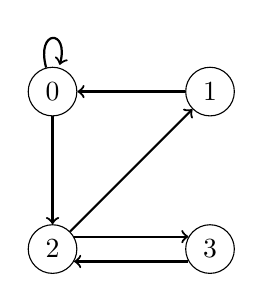
\begin{tikzpicture}
    \node[shape=circle,draw=black] (A) at (0,2) {0};
    \node[shape=circle,draw=black] (B) at (2,2) {1};
    \node[shape=circle,draw=black] (C) at (0,0) {2};
    \node[shape=circle,draw=black] (D) at (2,0) {3};
    \path  (A) edge [loop above, thick] (A);
    \path [->] (B) edge [thick] (A);  
    \path [->] (A) edge [thick] (C);  
    \path [->] (C) edge [thick] (B);  
    \path [->] (C.30) edge [thick] (D.150);  
    \path [->] (D.210) edge [thick] (C.-30);  
    \end{tikzpicture}
    \caption{The defined graph when $b = 4$. There are 4 nodes, each one corresponding to a value mod 4.}
    \label{fig:base_4_graph}
\end{figure}
There are 4 different nodes: one for each integer between 0 and 3. Because $4 = 2^2$, we are looking at the last 2 bits of each number. For example, a number congruent modulo to $0\Mod{4}$ has 00 as the 2 least significant bits, while a number congruent modulo to $2\Mod{4}$ has 10 as its 2 least significant bits. 
\subsubsection{Proof that base 4 graph is correct} \label{subsubsec:proofbase4graph}
Let us prove that this graph is correct.
\begin{theorem}
The base $4$ Collatz graph $G_4$, as shown in Figure~\ref{fig:base_4_graph}, is correct.
\end{theorem}
\begin{proof}
First, we will start with the even nodes, then the odd nodes:
\begin{itemize}
    \item Node 0 corresponds to the number ending with binary string ``00''. Removing the last 0 leaves either ``00'', looping to $0\Mod{4}$, or ``10'', changing it to $2\Mod{4}$.
    \item Node 2 corresponds to the number ending with binary string ``10''. Removing the last 0 leaves either ``01'', changing it to $1\Mod{4}$, or ``11'', changing it to $3\Mod{4}$.
\end{itemize}
Hence the even nodes and transitions from them are all correct. Now, the odd nodes:
\begin{itemize}
    \item Node 1 corresponds to the number ending with binary string ``01''. Multiplying this by 3 and adding 1 results in the binary number ending in ``$y_200$'', where $y_2$ is an unknown bit. Even though we don't know $y_2$, the number is still $0\Mod{4}$.
    \item Node 3 corresponds to the number ending with binary string ``11''. Multiplying this by 3 and adding 1 results in the binary number ending in ``$y_3y_210$'', which is still $2\Mod{4}$.
\end{itemize}
Hence, our graph is correct.
\end{proof}
\subsubsection{Base 4 subproblems} \label{subsubsec:base4subproblems}
We introduced the Base 4 case for nodes because we can prove that we need to visit all of the nodes in this graph. This is equivalent to saying that each of the Collatz Subproblems, $Col_{sub}(N,a,4)$ terminates
for $A = \{0\}$, $\{1\}$, $\{2\}$, or $\{3\}$, and for any input number $N$. 
\begin{theorem}
All vertices in the Collatz Base $4$ graph, $G_4$, are required.
\end{theorem}
\begin{proof}
We will start with proving that $Col_{sub}(N,2,4)$ will terminate for any input number $N$, because the 2 node is central to the graph.\par
\begin{lemma}
\label{lem:collatzSubTwoModFour}
$Col_{sub}(N,2,4)$ terminates for any $N$.
\end{lemma} 
\begin{proof}
We use the graph to help in this proof. A related question is this: Can we show that node 2 must be visited for all input numbers? To show that this is the case, we have to show that all other nodes must visit node 2. 
\begin{itemize}
    \item 2: If the input number is this, we are already done.
    \item 3: This must, by definition, transition after the $3x+1$ mapping has been applied in one step.
    \item 1 and 0: 1 must transition to 0 after applying the $3x+1$ mapping once. For 0, use Lemma~\ref{lem:zeroCycle}(the ``0 cycle'' lemma) for $b = 4$, and the number will eventually transition to the 2 node.
\end{itemize}
Hence, $Col_{sub}(N,2,4)$ terminates for any $N$.
\end{proof} \par

\begin{lemma}
\label{lem:collatzSubOneModFour}
$Col_{sub}(N,1,4)$ terminates for any $N$.
\end{lemma}
\begin{proof}
We use Lemma~\ref{lem:collatzSubTwoModFour} to show that we need to visit node 2, and Lemma~\ref{lem:oneConsumption} to show that the cycle between nodes 2 and 3 cannot continue indefinitely, so node 2 must eventually transition to 1, proving termination of this subproblem.
\end{proof}
\begin{lemma}
\label{lem:collatzSubZeroModFour}
$Col_{sub}(N,0,4)$ terminates for any $N$.
\end{lemma}
\begin{proof}
Given Lemma~\ref{lem:collatzSubOneModFour}, we know we must visit node 1, and given Lemma~\ref{lem:numOutEdges}, an odd node can only have one outgoing edge, so it must transition to node 0.
\end{proof}
\begin{lemma}
\label{lem:collatzSubThreeModFour}
$Col_{sub}(N,3,4)$ terminates for any $N$.
\end{lemma}
\begin{proof}
Given Lemma~\ref{lem:collatzSubTwoModFour}, we know we must visit node 2. Without node 3, the only cycle in the graph between nodes $2 \rightarrow 1 \rightarrow 0 \rightarrow 2$, including 0 cycles, would easily terminate for any number. This should lead to a theoretically easier proof of the Collatz Conjecture. So the $2 \rightarrow 3 \rightarrow 2$ cycle is needed to introduce hardness in solving the Collatz Conjecture, and is hence needed.
\end{proof}
Therefore, using all four of the provided lemmas, it is clear that all nodes are not only correctly in the base 4 graph, but are also required to represent the Collatz Conjecture from a base 4 perspective.
\end{proof}
\section{Base 8 Graph and Subproblems} \label{subsec:base8graphsubpblms}
We showed that the Base 4 graph is correct and that all nodes are necessary. We decided to see what would happen if we expanded to $k = 3$ bits. While we can build a graph and prove that it is correct, we are unable to formally prove the necessity of all of the nodes. This will motivate further computation undertaken in this paper, as we try to determine how hard figuring out these proofs are. \par
Figure~\ref{fig:base_8_graph} shows the base 8 graph.
\begin{figure}
    \centering
    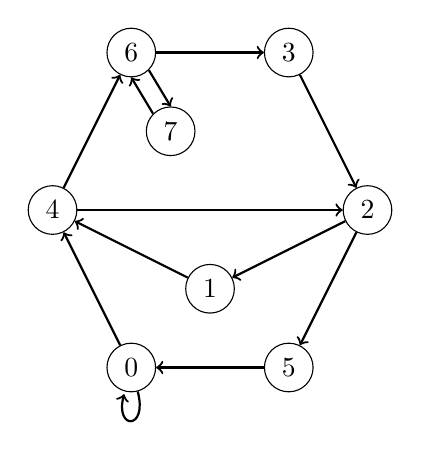
\begin{tikzpicture}
    \node[shape=circle,draw=black] (A) at (1,0) {0};
    \node[shape=circle,draw=black] (B) at (2,1) {1};
    \node[shape=circle,draw=black] (C) at (4,2) {2};
    \node[shape=circle,draw=black] (D) at (3,4) {3};
    \node[shape=circle,draw=black] (E) at (0,2) {4};
    \node[shape=circle,draw=black] (F) at (3,0) {5};
    \node[shape=circle,draw=black] (G) at (1,4) {6};
    \node[shape=circle,draw=black] (H) at (1.5,3) {7};
    \path  (A) edge [loop below, thick] (A);
    \path [->] (A) edge [thick] (E);  
    \path [->] (B) edge [thick] (E);  
    \path [->] (C) edge [thick] (B);  
    \path [->] (C) edge [thick] (F);  
    \path [->] (D) edge [thick] (C);  
    \path [->] (E) edge [thick] (C);  
    \path [->] (E) edge [thick] (G);  
    \path [->] (F) edge [thick] (A);  
    \path [->] (G) edge [thick] (D);  
    \path [->] (G.-45) edge [thick] (H.90);  
    \path [->] (H.135) edge [thick] (G.-90);  
    \end{tikzpicture}
    \caption{The defined graph when $b = 8$. There are 8 nodes, each one corresponding to a value mod 8.}
    \label{fig:base_8_graph}
\end{figure}
There are 8 different nodes. Because $8 = 2^3$, we are looking at the last 3 bits of each number. 
\subsection{Proof that base 8 graph is correct} \label{subsubsec:base8proof}
Like the base 4 graph, let us prove that the base 8 graph is correct:
\begin{theorem}
The base $8$ Collatz graph $G_8$, as shown in Figure~\ref{fig:base_8_graph}, is correct.
\end{theorem}
\begin{proof}
First, we have the right number of nodes, corresponding to all the possible integers that are the remainder after dividing by 8. Like in the base 4 case, let us examine the even nodes first. In this case, there are four different nodes: 0, 2, 4, and 6. Using Lemma~\ref{lem:numOutEdges}, each vertex has two different transitions, depending on what the next bit to the left of the 3 bits after removing the least significant 0. 
\begin{itemize}
    \item Node 0 corresponds to the binary string ``000''. Removing the last 0 leaves either ``000'', looping to $0\Mod{8}$, or ``100'', changing it to $4\Mod{8}$.
    \item Node 2 corresponds to the binary string ``010''. Removing the last 0 leaves either ``001'', changing it to $1\Mod{8}$, or ``101'', changing it to $5\Mod{8}$.
    \item Node 4 corresponds to the binary string ``100''. Removing the last 0 leaves either ``010'', changing it to $2\Mod{8}$, or ``110'', changing it to $6\Mod{8}$.
    \item Node 6 corresponds to the binary string ``110''. Removing the last 0 leaves either ``011'', changing it to $3\Mod{8}$, or ``111'', changing it to $7\Mod{8}$.
\end{itemize}
Hence the even nodes and transitions from them are all correct. Now, the odd nodes. Let $y_3$ and $y_4$ be unknown bits.
\begin{itemize}
    \item Node 1 corresponds to the binary string ``001''. Multiplying this by 3 and adding 1 results in the string ``100'', or $4\Mod{8}$.
    \item Node 3 corresponds to the binary string ``011''. Multiplying this by 3 and adding 1 results in the string ``$y_3010$'', which is $2\Mod{8}$.
    \item Node 5 corresponds to the binary string ``101''. Multiplying this by 3 and adding 1 results in the string ``$y_4y_3000$'', which is $0\Mod{8}$.
    \item Node 7 corresponds to the binary string ``111''. Multiplying this by 3 and adding 1 results in the string ``$y_4y_3110$'', which is $6\Mod{8}$.
\end{itemize}
So all of these transitions are correct as well, and our base 8 graph is correct.
\end{proof}
\subsection{Base 8 subproblems} \label{subsubsec:base8subprob}
As for which nodes we are forced to visit during the computation of a $3x+1$ sequence, we can conditionally prove needing to visit nodes 0, 2, 3, 4, and 6, but we don't have proofs for 1, 5, and 7. Here are how we know we must visit the 5 nodes we know:


\begin{itemize}
    \item \textbf{Node 0}: Needs to transition from $5\Mod{8}$. We can't totally prove this yet unless we prove the need for $5\Mod{8}$.
    \item \textbf{Node 2}: We can get to $2\Mod{8}$ in two different ways: Either from $3\Mod{8}$, which is needed, or directly from $4\Mod{8}$. So $2 \Mod{8}$ is definitely needed. 
    \item \textbf{Node 3}: Given Lemma~\ref{lem:oneConsumption}, a $6 \rightarrow 7 \rightarrow 6$ cycle cannot continue forever. Hence, $6\Mod{8}$ must transition to $3\Mod{8}$ eventually.
    \item \textbf{Node 4}: We know that we need $2\Mod{8}$ already. Both possible paths come from that node: Either we visit $1\Mod{8}$ then transition to $4\Mod{8}$, or we visit $5\Mod{8}$ then $0\Mod{8}$. From Lemma~\ref{lem:zeroCycle}, the 0 cycle cannot continue forever, so the number will eventually be $4\Mod{8}$.
     \marginnote{I do NOT like this explanation for Node 6. Needs to be retooled.}
    \item \textbf{Node 6}: If a $3x+1$ sequence never visited $6\Mod{8}$, it would be forced into one of two cycles: $4 \rightarrow 2 \rightarrow 1$ or $4 \rightarrow 2 \rightarrow 5 \rightarrow 0 \rightarrow \ldots \rightarrow 4$, where $\ldots$ is 0 or more repetitions of the 0 node being revisited. Both of these cycles cause the number to decrease in size, especially the second one, because both are dividing by at least 4 compared to the multiplication by 3. If all numbers followed these cycles, we would never have any numbers grow large in size, but we have several counterexamples showing that numbers do grow quite large, so hence, $6\Mod{8}$ must be visited as well.
   
\end{itemize}
1, 5, and $7\Mod{8}$ do not have proofs. All three numbers come from a even node, meaning each of these has two choices. Hence, we've run some computational experiments to try and better understand the difficulty of calculating these numbers as standalone nodes, and also as pairs. 
\subsection{Cycle analysis} \label{subsubsec:cycleanalysis}
In this section we provide a bit analysis of cycles in the base 8 graph, and show how several of these are equivalent to showing certain nodes are needed to be visited, and hence, how they tie to certain Collatz Subproblems.
\begin{itemize}
    \item The 0 self-cycle cannot continue forever, as per Lemma~\ref{lem:zeroCycle}.
    \item The $6 \rightarrow 7 \rightarrow 6$ cycle cannot continue forever as per Lemma~\ref{lem:oneConsumption}.
    \item The $4 \rightarrow 2 \rightarrow 1 \rightarrow 4$ cycle: Left blank, see margin note. \marginnote{Working on the $4 \rightarrow 2 \rightarrow 1 \rightarrow 4$ cycle, don't have a proof yet, but I think it's provable.}
    \item $4 \rightarrow 2 \rightarrow 5 \rightarrow 0 \rightarrow 4$ cycle: The proof for avoiding this cycle stems directly from the proof for node $6$ being required. This cycle can also include visits to node $1$ as well.
    \item $4 \rightarrow 6 \rightarrow 3 \rightarrow 2 \rightarrow 1 \rightarrow 4$ cycle: We don't have a proof for this cycle. Proving this doesn't hold and we have to break it is equivalent to proving that 5 and 7$\Mod{8}$ both cannot be avoided, a proof we explore in section~\ref{sec:subhrdnspred}. NOTE: If we allow visits to 7 in the cycle as well, then this proof would be equivalent to avoiding just $5 \Mod{8}$.
    \item $4 \rightarrow 6 \rightarrow 3 \rightarrow 2 \rightarrow 5 \rightarrow 0 \rightarrow 4$ cycle: There are three different variations to showing this cycle cannot continue forever, all of them unproven, and all of them lead to interesting questions.
    \begin{itemize}
        \item Allowing 7 but avoiding 1: This cycle is equivalent to showing why we need 1$\Mod{8}$. This proof might be challenging, because we'd have two conflicting cycles: one which causes the number to grow by 3/2 every time, and another one to divide by 2 every time. Our findings in section~\ref{sec:subhrdnspred} suggest this may be a cycle that grows in difficulty to find a proof as the numbers get larger.
        \item Allowing 1 but avoiding 7: This cycle is equivalent to the proof of why we need 7$\Mod{8}$. 
        \item Avoiding both 1 AND 7: This would be equivalent to the 1 and 7$\Mod{8}$ avoidance combination. We explore this combination in section~\ref{sec:subhrdnspred}.
    \end{itemize}
\end{itemize}

\chapter{Subproblem Hardness Prediction} \label{sec:subhrdnspred}
In this section, we attempt to determine how difficult subproblems from Algorithm~\ref{alg:ColSP} are for $Col_{sub}(N,A,8)$, where $A= \{1\}$, $\{5\}$, or $\{7\}$. We start by defining some measures, talk about the process how we ran experiments, and talk about the results, both analyzing avoidance of single nodes 1, 5, and 7, as well as pairs of these nodes.
\section{Defining Measures} \label{subsec:algdefinemeasure} 
We define hardness off of the notion that odd numbers make the Collatz Conjecture harder, whereas even numbers make it easier. To more precisely define the measures, define the following numbers, given some input number $x$:
\begin{itemize}
    %\item $x_i$: the number $x$ turns into after $i$ steps of the Collatz Mapping have been applied.
    \item $f(x)$: The total number of steps in the sequence for $x$ before it converges to 1.
    \item $f_\text{odd}(x)$: Number of odd numbers visited in the sequence from $x$ to 1.\footnote{If one wanted to figure out the number of visited even numbers, then $f_\text{even}(x) = f(x) - f_\text{odd}(x)$} 
    \item $A$: The base avoidance set, as defined in Algorithm~\ref{alg:ColSP}. For these subproblems, $A \subseteq \{1, 5, 7\}$ and $A \ne \varnothing$.
    \item $g(x,A)$: The highest number of steps, as an input number $x$ converges to 1, where $\forall a \in A$, $x_i \not\equiv a \Mod{8}$.
    \item $g_\text{odd}(x,A):$ The number of odd numbers within the given $g(x,A)$.
    \item A slice is a batch of numbers from some low number, denoted as $x_\text{low}$, to some high number, $x_\text{high}$.
    \item A record is any number $r$ in the range that has $g(r,A)$ higher than all numbers measured so far in the slice. More formally, any new record $r_\text{new}$ must have the properties compared to the current record $r_\text{current}$: $r_\text{new} > r_\text{current}$, and $g(r_\text{new},A) > g(r_\text{current},A)$ for a specific $A$. Note We measure records off of total steps, \textit{not} total number of odd numbers.
\end{itemize}
Using these numbers, two different measures are defined, and the intuition behind why they were chosen is given as well: \par
\textbf{Hardness}: Defined to be $H(x,A) = \frac{g_\text{odd}(x,A)}{\log_2{x}}$. This assesses whether or not increasing the number of bits needed to represent the number $x$ changes the difficulty of determining a proof for 1, 5, or $7\Mod{8}$, or some pair of the three.  \par
Also define ``Classical Hardness'' as a comparison: $H_C(x) = \frac{f_\text{odd}(x)}{\log_2{x}}$. This computes $H$ with respect to the whole sequence, instead of trying to avoid specific numbers. Records for Classical Hardness occur when $r_\text{new} > r_\text{current}$ and $f(r_\text{new}) > f(r_\text{current})$. \par
\textbf{Percentage of Sequence}: Defined to be $P(x,A) = \frac{g_\text{odd}(x,A)}{f_\text{odd}(x)}$. This assesses what percentage of all odd numbers lie within the longest sequence avoiding 1, 5, or $7\Mod{8}$, or some combination of the three.

\section{Generating Results} \label{subsec:algcomp}
I wrote a program that computed Collatz Sequences using Java, and ran it on all odd numbers from 1 to 1 billion. The program has various modes which evolved over the lifetime of this project. In these modes, let $\mathcal{A}$ be a family of avoidance sets $A$ we wish to compute, and let $x_{lowest}$ denote the lowest number in any slice, whereas $x_{highest}$ denotes the highest number in any slice.
\begin{itemize}
    \item baseavoid is the default option. This allows us to check all $A \in \mathcal{A}$ by running through all odd numbers from a given minimum (we usually use 1) to a given maximum (we usually use 1 billion), and determines the maximum number of steps we can run Algorithm~\ref{alg:ColSP} for each set $A$, or in other words, compute $g(x,A)$ for all odd $x$ in the range $x_{lowest} \leq x \leq x_{highest}$. When it finishes, it prints out the longest sequence for each $A$.
    \item entirechain just runs Algorithm~\ref{alg:ColR} for all odd $x$ in the range $x_{lowest} \leq x \leq x_{highest}$, and prints out the longest sequence.
    \item untildecay means that, for each odd number in between $x_{lowest}$ and $x_{highest}$, we continue to run until we have a number lower than the original number. We return only the longest sequence of numbers that occurs until the resulting number is smaller than the initial number.
    \item updown is a quite different mode. For each odd number $x$ such that $x_{lowest}\leq x \leq x_{highest}$, determine two things. First, the number of steps it takes for $x$ to become some number $x_i$ such that $x_i < x$. Second, the number of steps it takes for another number $x_g$ to grow to $x$ if such an $x_g$ exists (no multiple of 3 can grow from a smaller number, for instance). The output prints out, for all odd numbers in the range, $x_i$, the number of steps it takes for $x$ to turn into $x_i$, $x_g$ (if it exists), and the number of steps it takes for $x_g$ to grow into $x$, if $x_g$ exists.
    \item avoidingmodgrowth is a mode like baseavoid. However, it prints tables showing progressively growing records. This is the mode we used most often in this Thesis.
\end{itemize}
As mentioned, we used the avoidingmodgrowth mode to generate the records defined in subsection~\ref{subsec:algcomp}. We run for sequences of odd numbers in multiple slices, usually 8, in order to take advantage of parallel computing via a distributed computing program called Condor that was made by The University of Wisconsin-Madison~\cite{Thain:2005:DCP:1064323.1064336}, and combine the records of these 8 tables by hand. \par
We run sequences of numbers and have an option to avoid recomputing already seen odd numbers, as previously seen odd numbers will not generate new records. However, this option can be disabled if we wish to compute extremely large numbers and slices, and are limited in our memory storage. \par
The program could have been rewritten to build off of previously used results, which should run faster, but this might have been very tight on space and difficult without many GBs of memory available. So the space efficient approach was chosen for this project.
\section{Single Base Avoidance Analysis} \label{subsec:algsinglebase}
Our analysis for analyzing the avoidance of the nodes 1, 5, and 7 individually is broken into three subsections: Two exploring our defined computations, $H$ and $P$, and a third one analyzing interesting properties of sequence similarities.
For exploring $H$ and $P$, we took all of the records for $1 \Mod{8}$, $5 \Mod{8}$, and $7 \Mod{8}$, and plotted the log of all records $r$ versus $H(x,A)$ and $P(x,A)$, respectively. We also added in $3 \Mod{8}$ as a reference for both of these measures as a control case.
\subsubsection{Hardness Function Results and Analysis} \label{subsubsec:algsinhardness}
Figure~\ref{fig:hvslog} shows the results of $H(x,A)$ versus the number of bits ($\log_2{x}$). Total steps for each mod number were also added in as well.\par
\begin{figure}
    \centering
    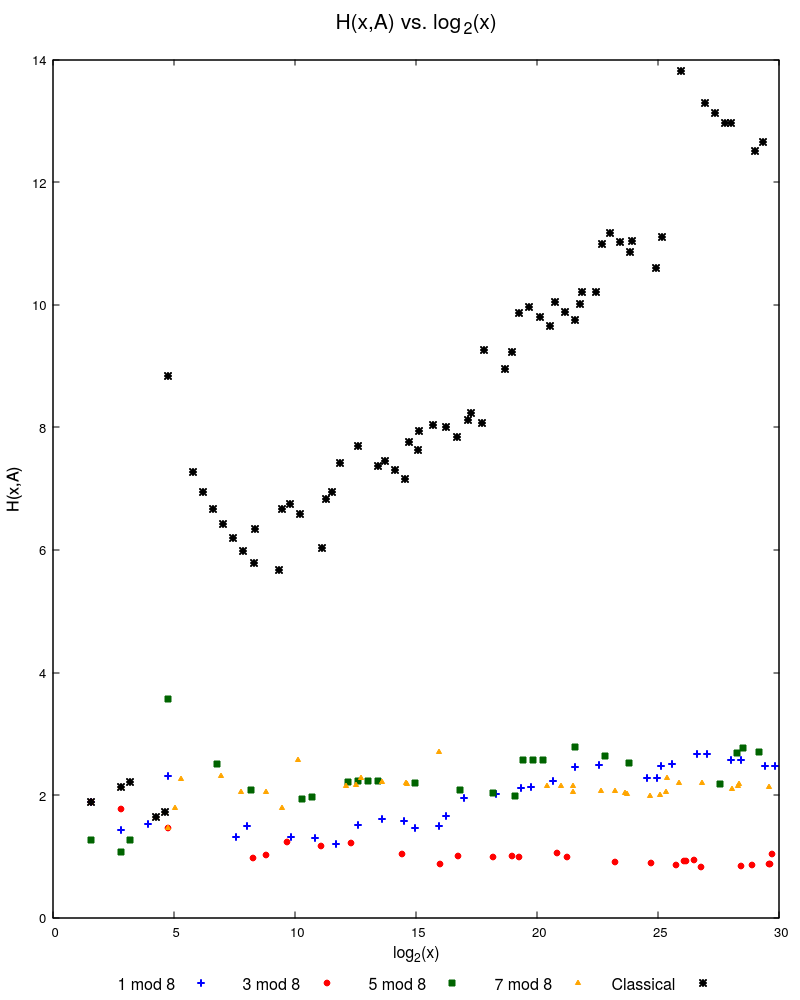
\includegraphics[scale=0.75]{ModAvoidanceAnalysisPics/H_vs_log.png}
    \caption{This graph visualizes how the $H$ values for $1 \Mod{8}$, $5 \Mod{8}$, and $7 \Mod{8}$ compare to each other, and to classical hardness. The log of the record holding numbers, or number of bits needed, is the x-axis, and the hardness measure $H$ as defined in subsection~\ref{subsec:algdefinemeasure} is the y-axis.}
    \label{fig:hvslog}
\end{figure}
Comparing the three unknown mods (1,5, and $7 \Mod{8}$) to the known mod ($3 \Mod{8}$), the known mod case is easier. The known mod case actually slight decreases in hardness as the number of bits increases, meaning that there are fewer odd numbers per bit than the unknown cases. \par
Comparing the unknown cases to themselves, there is no consistent leader among the three as the number of bits increases. However, they all seem to be around within a hardness range of 1-3, with only a couple of exceptions. $7 \Mod{8}$ seems to remain in the same range with no definite increase or decrease, whereas 1 and $5 \Mod{8}$ grow slightly from around 12 bits onward. The growth for both 1 and $5 \Mod{8}$ may be because as numbers get larger, there are more opportunities to visit the $6 \rightarrow 7 \rightarrow 6$ cycle, which rapidly adds more odd numbers. More experiments for higher numbers may need to be run in order to determine whether any of these three unknown cases trend the same way as we add more bits into the computation.
\marginnote{I think an appendix with the table results would at least be a good idea. Printing all the  sequences would be overkill.}
Classical Hardness actually tends to grow linearly against the log scale, meaning that as the input number increases, determining if the input number converges to 1 gets logarithimcally harder. This contrasts to all three mod cases, which tend to stay between values of 1.5 and 3 for $H$ for numbers below 1 billion, meaning that figuring out proofs for their need in the base 8 graph should be easier than proving the Collatz Conjecture.
\subsubsection{Percentage of Sequence Function Results and Analysis} \label{subsubsec:algsinpercentage}
 Figure~\ref{fig:pvslog} shows the results of $P(x,A)$ versus the number of bits.\par 
\begin{figure}
    \centering
    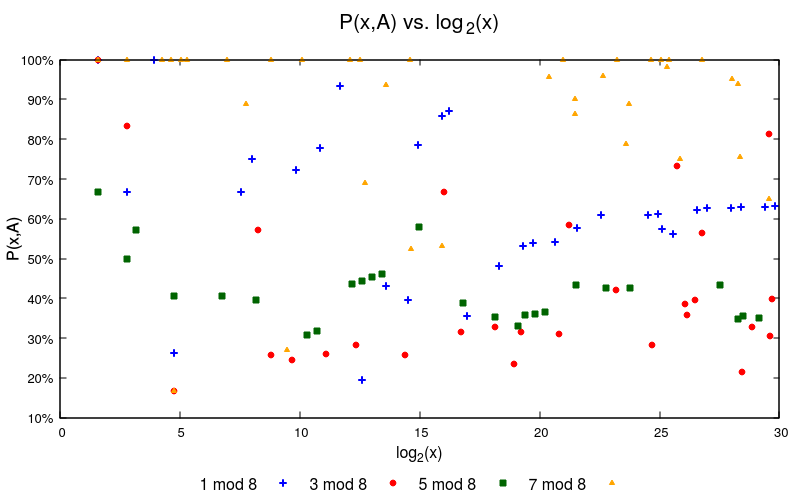
\includegraphics[scale=0.75]{ModAvoidanceAnalysisPics/P_vs_log.png}
    \caption{This graph visualizes how the $P$ values for $1 \Mod{8}$, $5 \Mod{8}$, and $7 \Mod{8}$ compare to each other. The log of the record holding numbers, or number of bits needed, is the x-axis, and the percentage measure $P$ as defined in subsection~\ref{subsec:algdefinemeasure} is the y-axis.}
    \label{fig:pvslog}
\end{figure}

$P(x,A)$, as discussed earlier, is just calculating what percentage of the record sequence contributes to the overall decay of that sequence to 1. \par
Avoiding $7 \Mod{8}$ has the highest percentage overall, with a couple of exceptions. Avoiding $7 \Mod{8}$ causes the sequence to decline rapidly, since the $6 \rightarrow 7 \rightarrow 6$ cycle causes an input number to grow faster than any other cycle in the base 8 graph. Almost all of the records avoiding $7 \Mod{8}$ terminate at 1 instead of actually reaching a number that is $7 \Mod{8}$. \par
Likewise, avoiding $5 \Mod{8}$ tends to have a low percentage overall, and is the least erratic of all four nodes, meaning the standard deviation is lower. Avoiding $5 \Mod{8}$ avoids the 0 self-cycle, which causes many divisions by 2. Numbers having a long sequence of avoiding $5 \Mod{8}$ tend to have a very large number when they hit $5 \Mod{8}$, meaning that often, many more steps in the $3x+1$ mapping must be taken before these numbers converge to 1. \par
$1 \Mod{8}$ is interesting, because as the input numbers grow larger, the line changes from erratic behavior to a more steady percentage between approximately 50\% and 60\% at around 20 bits. This is likely a consequence of the sequence similarity that is seen in larger record sequences that avoid $1 \Mod{8}$, which will be analyzed in subsubsection~\ref{subsubsec:algseqsim}. Further, as mentioned in the cycle analysis for the $4 \rightarrow 6 \rightarrow 3 \rightarrow 2 \rightarrow 5 \rightarrow 0 \rightarrow 4$ cycle (allowing $6 \rightarrow 7 \rightarrow 6$, but avoiding 1), avoiding $1\Mod{8}$ causes a clash between the decay of the 0 self-cycle and the growth of the $6 \rightarrow 7 \rightarrow 6$ cycle, which may explain some of the erratic behavior for $1\Mod{8}$, aside from chain similarity.
$3 \Mod{8}$ tends toward the lowest percentage of all odd numbers, even lower than $5 \Mod{8}$, but also has erratic behavior. This could be explained by the fact that avoiding $3 \Mod{8}$ causes the sequence to follow some combination of the $6 \rightarrow 7 \rightarrow 6$ cycle, the $4 \rightarrow 2 \rightarrow 1 \rightarrow 4$ cycle, or the $4 \rightarrow 2 \rightarrow 5 \rightarrow 0 \rightarrow 4$ cycle with some number of $0$ self-cycles. The first cycle causes growth, whereas all three other cycles cause decay. If the growth cycle is followed, the percentage tends to be lower as the number gets larger, whereas the decay cycles cause the number to shrink, tending the percentages to be higher. This may explain why avoiding $3 \Mod{8}$ causes widely different percentages.
\subsubsection{Sequence similarity analysis} \label{subsubsec:algseqsim}
We analyzed the sequences of the records for 1, 5, and 7 $\Mod{8}$ as well to see if we could find any similarities:
\begin{itemize}
    \item $1\Mod{8}$: There are two groups of records that were particularly interesting: Those from 325,791 to 32,505,681 (call this group $S$), and those from 35,651,835 to 949,643,331 (call this group $T$). Group $S$ numbers all terminated at number 161, and group $T$ numbers all terminated at number 35,369. These sequences all matched \textbf{number-by-number} at least one other sequence starting at most 8
    steps from the beginning. This is a striking similarity meaning that records avoiding $1 \Mod{8}$ might be predictably related to groups $S$ or $T$, or perhaps to other groups.
    \item $7 \Mod{8}$: All record sequences, except for input number 27, terminated at 1. While there was some similarity between sequences (all numbers $\geq 62079$ had the same last 41 numbers), there were many different paths taken from the input, so not as many patterns here.
    \item $5 \Mod{8}$: This had few matches and was the most changing of the records, so it was difficult to pin down any pattern.
\end{itemize}
\section{Paired Base Avoidance Analysis} \label{subsec:algpairedbase}
Because it appears to be difficult to figure out why there is a need for the bases 1, 5, and 7 individually, we have also analyzed pairs of them. Hence, we are trying to find termination of Algorithm~\ref{alg:ColSP} for $|A| = 2$ sets. This section will analyze what happens to $H(x,A)$ and $P(x,A)$ where $A$ is equal to three different base sets: $\{1,5\}$, $\{1,7\}$, and $\{5,7\}$. We already have a straightforward proof for when $A = \{1, 5\}$: Given Lemma~\ref{lem:oneConsumption}, the $6 \rightarrow 7 \rightarrow 6$ cycle can't go on forever, meaning the sequence must eventually follow to $3 \rightarrow 2$, then either 1 or 5. We still included that result to compare it to the other two types of hardness we do not have proofs for: when $A = \{1,7\}$ and $A = \{5,7\}$.

\subsection{Hardness Function Results and Analysis} \label{subsubsec:algmulhardness}
Figure~\ref{fig:h_multivslog} shows the results of $H(x,A)$ versus $\log_2{x}$. Total steps for each mod number were also added in as well.\par
\begin{figure}

    \centering
    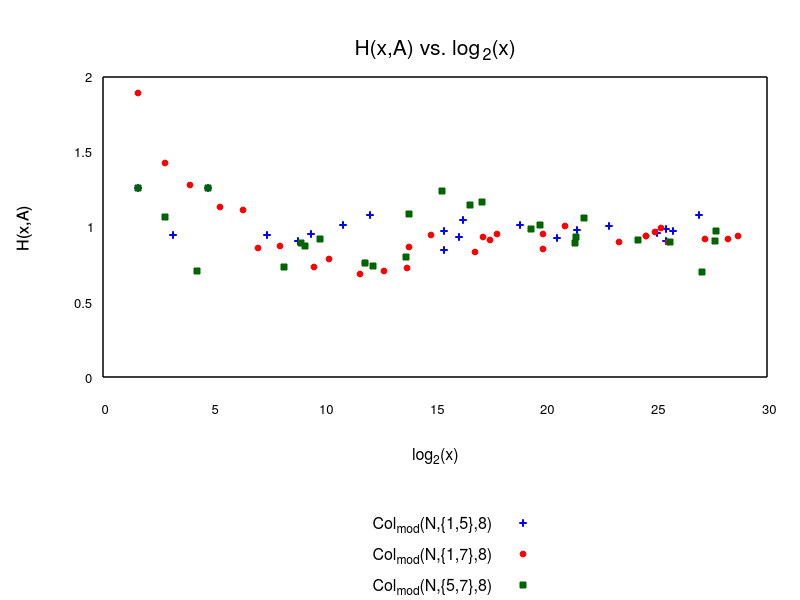
\includegraphics[scale=0.75]{ModAvoidanceAnalysisPics/H_vs_log_multi_base.png}
    \caption{This graph visualizes the $H$ measure for three pairs of avoidance bases for when $A = \{1,5\}$, $A= \{1,7\}$, and $A = \{5,7\}$. The log of the record holding numbers, or number of bits needed, is the x-axis, and the hardness measure $H$ as defined in subsection~\ref{subsec:algdefinemeasure} is the y-axis. Classical Hardness was omitted from this graph to eliminate distortion.}
    \label{fig:h_multivslog}
\end{figure}
These results shocked us. At first thought, it would have appeared that $A = \{1, 5\}$ should be the easiest to determine, because we already had a proof for it. But both $A = \{1, 7\}$ and $A = \{5, 7\}$  had alike predictive hardness to $A = \{1, 5\}$! These numbers suggest that a proof for determining why numbers cannot avoid both $A = \{1, 7\}$, as well as $A = \{5, 7\}$, either should be closer than we anticipated, or our hardness measures are not very good. However, given the fact that $3\Mod{8}$ for the single base cases is clearly easier than 1, 5, or 7 $\Mod{8}$, we have reason to believe this measure should be good. Further investigation needs to be considered.


\subsection{Percentage of Sequence Function Results and Analysis} \label{subsubsec:algmulpercentage}
Figure~\ref{fig:p_multi_vslog} shows the results of $P(x,A)$ versus $\log_2{x}$.\par
\begin{figure}
    \centering
    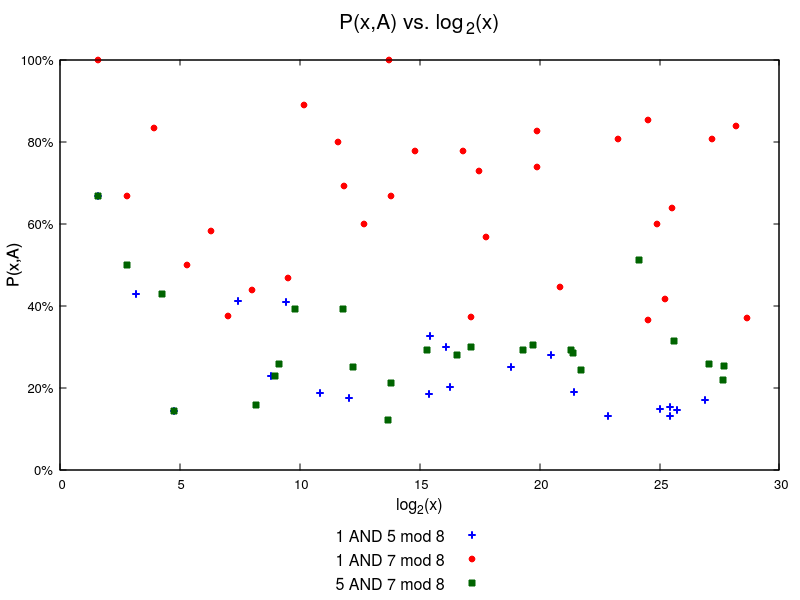
\includegraphics[scale=0.75]{ModAvoidanceAnalysisPics/P_vs_log_multi_base.png}
    \caption{This graph visualizes the $P$ measure for three pairs of avoidance bases for when $A = \{1,5\}$, $A= \{1,7\}$, and $A = \{5,7\}$. The log of the record holding numbers, or number of bits needed, is the x-axis, and the hardness measure $P$ as defined in subsection~\ref{subsec:algdefinemeasure} is the y-axis.}
    \label{fig:p_multi_vslog}
\end{figure}
The avoidance pair $A= \{1,7\}$ makes up the highest percentage of the sequence compared to the other two cases, because avoiding both the $6 \rightarrow 7 \rightarrow 6$ and the $4 \rightarrow 6 \rightarrow 3 \rightarrow 2 \rightarrow 1$ cycles only allows for the sequence to go to $5\Mod{8}$, which causes it to hit the 0 cycle, causing fast decay, like in the $7\Mod{8}$ case. \par
Both of the avoidance pairs $A= \{1,5\}$ and $A= \{5,7\}$ are much closer to each other in percentage of total sequence, although as the numbers grow past 17 bits in size, $A= \{5,7\}$ comprises of the higher percentage of the sequence. A possible explanation is the fact that the $6 \rightarrow 7 \rightarrow 6$ cycle allowed in $A = \{1,5\}$ allows causes a number to grow larger than the $4 \rightarrow 6 \rightarrow 3 \rightarrow 2 \rightarrow 1$ cycle that $A= \{5,7\}$ allows does, and since $A = \{1,5\}$ allows for larger numbers, and the fact that larger numbers generally (but not always) take more steps to decline, that allowing for more growth should mean that the long avoidance sequence for $A = \{1,5\}$ should make up a lower percentage of all odd numbers.


\chapter{SAT Solving Background} \label{sec:SATsolving}
We want to not only analyze the hardness for the Collatz Subproblems from an algebraic perspective, but from a String Rewrite System perspective too. The next two sections deal with background required for explaining the rewrite system approach using SAT solvers, which justifies the hardness measures discussed later in this paper. First, this section will talk about the background of Boolean satisfiability, Boolean constraint propagation (BCP), the power of splitting heuristics, and the cube-and-conquer paradigm. Then, section~\ref{sec:SRSandSAT} will talk about String Rewrite Systems and how SAT solvers can be used to solve termination of them.

\section{Boolean satisfiability} \label{subsec:boolSAT}
A Boolean formula $F$ is a formula that has inputs and outputs of values true ($\boldsymbol{t}$) or false ($\boldsymbol{f}$). The base of a Boolean formula is called an atom, which is either a propositional variable, or the truth values $\boldsymbol{t}$ or $\boldsymbol{f}$. Let $p$ be a propositional variable. A literal is modifying an atom to get one of two different types: $p$, the atom itself, is a positive literal, and $\Bar{p}$  is a negative literal. A truth assignment to a formula $F$ is a partial function $\tau$ that maps literals in $F$ to $\{\boldsymbol{t}, \boldsymbol{f}\}$. \par
SAT Solvers work with a very specific type of Boolean formula called \textit{Conjunctive Normal Form} (CNF). A CNF formula only uses three Boolean operators: AND ($\wedge$), OR ($\vee$) and NOT (a negative literal or $\neg$). In a CNF formula, a clause is a disjunction of literals (disjunction meaning literals are all ORed together). The whole formula is a conjunction of clauses (conjunction meaning clauses are all ANDed together). SAT solvers work with CNF formulas because all Boolean Formulas can be converted to CNF with only a polynomial size increase due to Tseitin's Transformation~\cite{Tseitin70}. \par
Given a CNF formula $F$ and truth assignment $\tau$, the following things are true:
\begin{itemize}
    \item A clause $C$ is \textit{satisfied} by $\tau$ if $\tau(l) = \boldsymbol{t}$ for some $l \in C$
    \item A clause $C$ is \textit{falsified} by $\tau$ if $\tau(l) = \boldsymbol{f}$ for all $l \in C$
    \item A formula $F$ is \textit{satisfied} by $\tau$ if $\tau(C) = \boldsymbol{t}$ for all $C \in F$
    \item A formula $F$ is \textit{falsified} by $\tau$ if $\tau(C) = \boldsymbol{f}$ for some $C \in F$
\end{itemize}
The Boolean satisfiability problem (or SAT for short) asks whether a CNF formula contains a satisfying assignment. If a formula has a satisfying assignment, then the formula is \textit{satisfiable}. Otherwise, the formula is \textit{unsatisfiable}. $k$-SAT, where $k$ is the maximum number of literals per clause, is a decision problem derived from SAT that is NP-Complete when $k > 2$, meaning that if $P \ne NP$, the worst case runtime is exponential. However, with clever heuristics, we can actually make CNF formulas run in linear time for many interesting cases. As a result, SAT solvers can solve some incredibly complex problems, such as those found in hardware verification, software verification, and combinatorics.

\section{Boolean Constraint Propogation (BCP)} \label{subsec:BCP}
For a clause $C$ in a CNF formula $F$, we say that it is in \textit{unit} if, given an assignment $\tau$, there exists a literal $l \in C$ such that $l \not\in \tau$ and $\Bar{l} \not\in \tau$, and for all other literals $l' \in C$ such that $l' \ne l$, $\Bar{l'} \in \tau$. In other words, all literals besides one in $C$ have been assigned a truth value already that don't satisfy the clause $C$. Since $F$ is falsified if even one clause is falsified, we know that $l$ must be given the truth value that satisfies $C$. So if $l \in C$, then $l = \boldsymbol t$, and if $\Bar{l} \in C$, then $l = \boldsymbol f$. 
Boolean Constraint Propagation (BCP) takes some assignment, and extends it by finding unit literals with forced assignments using what is called \textit{unit resolution}. It continues to extend the assignment until it can no longer be extended, either when $F$ is satisfied, $F$ is falsified, or no forced unit literals need be assigned. If the assignment falsifies $F$, we say that BCP derived a conflict. \par
As SAT solvers use heuristics to determine assignments (see subsection~\ref{subsec:BCP}), they use BCP as their main inference mechanism. Algorithm~\ref{alg:BCP} shows the steps that a SAT solver takes after an assignment $\tau$ has been set on a formula $F$. As shown in this algorithm, BCP continues to extend unit literals until the formula has no more unit clauses, or a conflict has been derived. 
\begin{algorithm}
\caption{$BCP(F, \tau)$}
\label{alg:BCP}
\begin{algorithmic}[1]
    \Require $F$ is set of CNF clauses, $\tau$ is an assignment of literals
    \Ensure Either a pair ($F$, $\tau$) of the modified formula, or $\bot$ if conflict derived
    \While{$F$ contains a unit clause $(l)$}
        \If{$(\Bar{l}) \in F$}
            \Return $\bot$ \Comment{Clause $\Bar{l}$ in formula, conflict derived}
        \EndIf
        \State Add $l$ to $\tau$
        \State Remove all clauses containing $l$ from set $F \backslash \{(l)\}$
        \State Remove literal $\Bar{l}$ from all clauses in $F$
    \EndWhile
    \State \Return ($F$, $\tau$)
\end{algorithmic}
\end{algorithm}

\section{The power of splitting heuristics} \label{subsec:splitheur}
For some simpler problems, using brute force and enumerating all cases is possible. However, there are some problems that have so many combinations that it would be impossible to solve on a computer. Hence, SAT solvers use heuristics aiming to exponentially reduce the search space. However, the intuition of knowing which heuristics work best for certain problems makes SAT solving challenging as a whole. To illustrate the power of splitting heuristics, let us first consider a problem with a simple answer, then we will talk about a problem with a much more complex, and famous, answer.\par
The first problem is called the Boolean Schur Triples problem, and asks whether the natural numbers $\{1, 2, \ldots \}$ can avoid being colored monochromatically red or blue in the equation $a + b = c$, such that $a < b < c$. The answer is no, because it is not possible to color the numbers $\{1, \ldots, 9\}$ monochromatically. To show this using brute force, one would have to enumerate all possible numerical combinations up to 9: $2^9 = 512$ different colorings. However, we can use the following encoding of the 9 case that forces one summation of the numbers to be monochromatic:
\begin{align*}
(x_1 \vee x_2 \vee x_3 ) &\wedge ( \overline{x}_1 \vee \overline{x}_2 \vee \overline{x}_3 ) \wedge (x_1 \vee x_3 \vee x_4 ) \wedge ( \overline{x}_1 \vee \overline{x}_3 \vee \overline{x}_4 ) \wedge \\
(x_1 \vee x_4 \vee x_5 ) &\wedge ( \overline{x}_1 \vee \overline{x}_4 \vee \overline{x}_5 ) \wedge (x_2 \vee x_3 \vee x_5 ) \wedge ( \overline{x}_2 \vee \overline{x}_3 \vee \overline{x}_5 ) \wedge \\
(x_1 \vee x_5 \vee x_6 ) &\wedge ( \overline{x}_1 \vee \overline{x}_5 \vee \overline{x}_6 ) \wedge (x_2 \vee x_4 \vee x_6 ) \wedge ( \overline{x}_2 \vee \overline{x}_4 \vee \overline{x}_6 ) \wedge \\
(x_1 \vee x_6 \vee x_7 ) &\wedge ( \overline{x}_1 \vee \overline{x}_6 \vee \overline{x}_7 ) \wedge (x_2 \vee x_5 \vee x_7 ) \wedge ( \overline{x}_2 \vee \overline{x}_5 \vee \overline{x}_7 ) \wedge \\
(x_3 \vee x_4 \vee x_7 ) &\wedge ( \overline{x}_3 \vee \overline{x}_4 \vee \overline{x}_7 ) \wedge (x_1 \vee x_7 \vee x_8 ) \wedge ( \overline{x}_1 \vee \overline{x}_7 \vee \overline{x}_8 ) \wedge \\
(x_2 \vee x_6 \vee x_8 ) &\wedge ( \overline{x}_2 \vee \overline{x}_6 \vee \overline{x}_8 ) \wedge (x_3 \vee x_5 \vee x_8 ) \wedge ( \overline{x}_3 \vee \overline{x}_5 \vee \overline{x}_8 ) \wedge \\
(x_1 \vee x_8 \vee x_9 ) &\wedge ( \overline{x}_1 \vee \overline{x}_8 \vee \overline{x}_9 ) \wedge (x_2 \vee x_7 \vee x_9 ) \wedge ( \overline{x}_2 \vee \overline{x}_7 \vee \overline{x}_9 ) \wedge \\
(x_3 \vee x_6 \vee x_9 ) &\wedge ( \overline{x}_3 \vee \overline{x}_6 \vee \overline{x}_9 ) \wedge (x_4 \vee x_5 \vee x_9 ) \wedge ( \overline{x}_4 \vee \overline{x}_5 \vee \overline{x}_9 )
\end{align*}
Variable $x_n$ represent number $n$. $x_n$ means color number $n$ red, whereas $\overline{x}_n$ denotes to color number $n$ blue. Each clause is saying any one of three numbers $a$, $b$, or $c$ where $a + b = c$ must be colored either red or blue. \par
We can use a heuristic to choose a good variable to reduce the search space by a large size. The  heuristic chooses a variable in which we have cases where we set the variable to both true and false. We can apply the Maximum Occurrences of Minimal Size (MOMS) heuristic, and reduce the number of cases from 512 to 6. On the first step, all clauses are of size 3, so we choose $x_1$ because it occurs in the most clauses. We can set $x_1$ to true. As discussed, we remove all clauses which have $x_1$, and remove all occurrence of $\overline{x}_1$ from remaining clauses. The resulting formula does not apply BCP yet, because we have no unit clauses. Now we look at MOMs and several variables are in clauses of length 2, but we apply a tiebreak: which variable are in the most clauses of length 3? The answer is $x_3$. We, hence, set that to true. Now BCP finds that $x_2$ and $x_4$ must be set to false ($1+2 = 3$ and $1+3 = 4$), which forces $x_6$ to be true ($2+4=6$), which forces $x_7$ and $x_9$ to be false ($1+6 = 7$ and $3+6 = 9$). However, $2+7=9$, and all those numbers are false, so $x_3$ can't be true. So now the SAT solver sets $x_3$ to false. This time, no more BCP can be applied. The resulting clause runs MOMs and finds that $x_5$ occurs in the most clauses with length 2. Setting this to true forces 4 and 6 to be false ($1+4 = 5$ and $1+5 = 6$), which forces 2 and 7 to be true ($2+4=6$ and $3+4=7$). However, this makes $2+5 = 7$ all true, leading to another contradiction. Switching $x_5$ to false also leads to a contradiction, and backtracking and switching $x_1$ to false also clearly leads to a contradiction, and trying to once again set $x_3$ then $x_5$ to true and false, also leading to contradictions. This is a total of 6 variable assignments, much fewer than the 512 that brute force would have enumerated. \par
For this case, MOMS was a great choice, but it is one of many heuristics. We will talk about two more examples. One is called Dynamic Largest Individual Sum (DLIS)~\cite{Silva:1999:IBH:645377.651196}, which targets literals that satisfy the most number of clauses. Going back to our example using this heuristic, we would choose either $x_1$ or $\overline{x}_1$ (both are tied) and assign the values that way. Another example is called Variable State Independent Decaying Sum (VSIDS)~\cite{Moskewicz:2001}. This heuristic favors variables that are stored in more conflict clauses, a big part of Conflict-Driven Clause Learning (CDCL), which will be covered more in subsection~\ref{subsec:cnc}. \par
The Boolean Schur Triples problem is a very simple case, but heuristics on a larger scale are much more impressive. Famously in 2016, Heule, Kullmann, and Marek solved the Pythagorean Triples Problem using SAT solving, producing a 200 TB proof, the largest ever at the time~\cite{DBLP:journals/corr/HeuleKM16}. The Pythagorean Triples Problem is like the Boolean Schurs problem, but instead asks it is possible to avoid a monochromatic coloring of three natural numbers such that $a^2+b^2 = c^2$. The answer determined was that it is possible up to 7824, but not possible for 7825. To confirm that the number is 7825 with just brute force, it would take $2^{7825}$ different cases, which is over $2^{7000}$ times the estimated number of particles in the universe! With heuristics, it is possible to reduce the number of cases to around a trillion $(\sim 2^{40})$, which, while still a huge amount of cases, was solvable in a few CPU years, much better than the immeasurable amount of power brute force would require.

\section{Cube-and-Conquer} \label{subsec:cnc}
Cube-and-Conquer is a SAT solving paradigm developed by Heule, Kullman, Wierigna, and Biere~\cite{HeuleKWB12} that was famously applied to the Pythagorean Triples Problem~\cite{DBLP:journals/corr/HeuleKM16}. Cube-and-Conquer splits a problem into $N$ problems using heuristics. There are two different phases to Cube-and-Conquer: The ``Cube'' phase, which partitions the problems into $N$ problems using a look-ahead solver, and the ``Conquer'' phase, which solves these problems using a CDCL (Conflict Driven Clause Learning) solver. This section will talk about each phase in a bit more detail. 

\subsection{``Cube'' phase} \label{subsubsec:cnccube}
A ``Cube'' is a conjunction of literals. It can be disjuncted with several other cubes, creating a formula in DNF. If one of the cubes is satisfied, then the DNF formula is satisfied. \par
Such is the underlying notion of the ``Cube'' phase of Cube and Conquer. A lookahead solver uses the David-Putnam-Logemann-Loveland (DPLL) algorithm~\cite{Davis:1962:MPT:368273.368557}. The DPLL algorithm assigns a literal $x_1 = \boldsymbol t$ then applies BCP until a conflict is derived, or another literal needs to be assigned a value. Lookahead solvers use the assignment of a literal to a formula $F$, apply BCP if needed, then derive a new formula $F'$, then finally, it measures the difference between $F$ and $F'$ to determine if $x_1$ was a good variable choice.  Then, given $n$ literal selections, the cube $C = x_1 \wedge x_2 \cdots \wedge x_n$ is built. If a conflict is derived when solving $C$, then we know the negation of this cube, $\overline{C}$, must be true. The negation of a cube can also be used as a conflict clause. \par
$N$ (valid) cubes are built, and the reduced subformulas $\{F'_1, \ldots, F'_N\}$ are hence fed to the ``Conquer'' phase. The optimal $N$ that should be built for the fastest runtime varies from problem to problem, and is in essence a decision heuristic of its own.

 \subsection{``Conquer'' phase} \label{subsubsec:cncconquer}
 A CDCL SAT Solver learns conflict clauses by deriving conflicts from BCP. For instance, if $x_1 = \boldsymbol t$, $x_2 = \boldsymbol f$, and $x_3 = \boldsymbol f$ leads to a conflict in $F$, then CDCL derives a conflict clause of $\overline{(x_1 \wedge \overline{x_2} \wedge \overline{x_3})} = (\overline{x_1} \vee x_2 \vee x_3)$ by DeMorgan's Law. Since this conflict clause must hold true for the overall CNF formula, we can append it to the CNF formula we are trying to solve, and prevent the SAT solver from straying towards incorrect variable selections again, reducing runtime. \par
 Combined with the ``Cube'' phase, in some cases, the $N$ subformulas created by the cubes can be refuted (or satisfied) much quicker than if the whole formula were to try and be solved using CDCL. Further, the subformulas can be parallelized quite easily to many different computers, making Cube and Conquer an attractive option for use with multicore computers.

\chapter{String Rewriting Systems (SRS) and SAT Solvers} \label{sec:SRSandSAT}
A string rewriting system (SRS), at a high level, takes a input string of an alphabet, and applies string rewriting rules (SRRs) in an arbitrary order on the input string to see if the string can be transformed further. An example SRS is given.
\begin{definition}{SRS A:} 
The alphabet is $\Sigma = \{a, b, c\}$ and the SRRs are as follows:
\begin{enumerate}
    \item $aa \rightarrow bc$
    \item $bb \rightarrow ac$
    \item $cc \rightarrow ab$
\end{enumerate}
\end{definition}
A problem, called Zantema's Other Problem~\cite{Hofbauer:2006:TA:1142725.1711178}, using SRS A, asks the following question:\par\noindent
\begin{question}{Zantema's Other Problem:}
Does the system laid out in SRS $A$ terminate for any input string $(a|b|c)*$?
\end{question}
If one thinks about this problem a little, it would seem that a proof to show that this problem terminates for all input strings should be easy to show. \marginnote{I'm unsure of whether I should go into more detail for this section.} Surprisingly, both humans and computers struggled to come up with a proof for this problem when initially presented.  However, Hofbuaer and Waldmann came up with a proof for determining that it terminates~\cite{Hofbauer:2006:TA:1142725.1711178}, and from this, found that, for any rewriting rules in any rewrite system, if they are transformed into functions that causes all inputs to decrease, then the rewrite system will terminate.~\cite{Hofbauer2006}. \par
The matrices are built using SAT solving to determine if a $d \times d$ matrix is large enough to ensure that the matrix functions for the set of rewrite rules always decrease for all inputs. The process of building these matrices is described in a paper by Endrullis, Waldmann and Zantema~\cite{Endrullis2006}. An example using Zantema's Other Problem will be explained here.\par
Here are the matrices computed by SAT from ~\cite{Hofbauer:2006:TA:1142725.1711178}:
%FIX THIS OVERFULL PROBLEM HERE AND IN THE NEXT SET.
\[
a(\Vec{x}) = \begin{pmatrix}
1&0&0&3\\
0&0&2&1\\
0&1&0&1\\
0&0&0&0
\end{pmatrix} \Vec{x} + \begin{pmatrix}
1\\
0\\
1\\
0
\end{pmatrix}
b(\Vec{x}) = \begin{pmatrix}
1&2&0&0\\
0&2&0&1\\
0&1&0&0\\
0&0&0&0
\end{pmatrix} \Vec{x} + \begin{pmatrix}
1\\
2\\
0\\
0
\end{pmatrix}
c(\Vec{x}) = \begin{pmatrix}
1&0&0&1\\
0&0&0&1\\
0&1&0&1\\
0&2&0&0
\end{pmatrix} \Vec{x} + \begin{pmatrix}
1\\
0\\
3\\
0
\end{pmatrix}
\]
We will show an example string to show that it is always decreasing, but first, we need to define an appropriate operator. Define the $\succ$ operator to show that, for vectors $(x_1 \ldots x_d)$ and $(y_1 \ldots y_d)$, $(x_1 \ldots x_d) \succ (y_1 \ldots y_d)$ if $x_1 > y_1$ and $x_i \geq y_i$ for $i \in \{2, \ldots, d\}$. In other words, the first element of a vector must be always decreasing, while the other $d-1$ elements must either be the same or decrease. \par
Let our sample string be $bbaa$. Here is a possible set of rules that can be applied to it as well as the vector representations of the symbols:
%FIX THIS OVERFULL PROBLEM HERE
\begin{align*}
    bb\underline{aa} &\rightarrow b\underline{bb}c &\rightarrow ba\underline{cc} &\rightarrow b\underline{aa}b &\rightarrow \underline{bb}cb &\rightarrow a\underline{cc}b &\rightarrow aa\underline{bb} &\rightarrow a\underline{aa}c &\rightarrow ab\underline{cc} &\rightarrow abab \\
    \begin{pmatrix}18\\14\\6\\0\end{pmatrix} &\succ
    \begin{pmatrix}17\\14\\6\\0\end{pmatrix} &\succ
    \begin{pmatrix}15\\14\\6\\0\end{pmatrix} &\succ
    \begin{pmatrix}14\\14\\6\\0\end{pmatrix} &\succ
    \begin{pmatrix}13\\14\\6\\0\end{pmatrix} &\succ
    \begin{pmatrix}7\\14\\5\\0\end{pmatrix} &\succ
    \begin{pmatrix}6\\14\\5\\0\end{pmatrix} &\succ
    \begin{pmatrix}4\\14\\3\\0\end{pmatrix} &\succ
    \begin{pmatrix}3\\0\\3\\0\end{pmatrix} &\succ
    \begin{pmatrix}2\\0\\3\\0\end{pmatrix}
\end{align*}
The vector representation of the strings are always decreasing as defined by the $\succ$ operator. We could apply any string with symbols $a$, $b$, and $c$ and apply rules until termination and the vectors representing the strings would always decrease.

\chapter{The Collatz Conjecture as a rewriting system} \label{sec:CollatzSRS}
Using the knowledge discussed in section~\ref{sec:SRSandSAT}, Aaronson built an SRS representing the Collatz Conjecture~\cite{HeuleAaronson}. We'll call this the Collatz SRS throughout the remainder of this Thesis. \par
Let the alphabet of the Collatz SRS consist of the symbols $a, b, c, d, e, f, g$. The symbols can be written as these linear functions:
\[
a(x) = 2x, b(x) = 2x+1, c(x) = 1, d(x) = x, e(x) = 3x, f(x) = 3x+1, g(x) = 3x+2
\]
%the binary symbols and ternary symbols part is a bit awkward, but decided to come back to it later.
The symbols $a$ and $b$ are binary symbols. They represent  a binary system: $a$ is 0 and $b$ is 1.  The symbols $e$, $f$, and $g$ are ternary symbols. They represent a ternary system: $e$ is 0, $f$ is 1, and $g$ is 2. $c$ and $d$ are placeholder symbols to represent the leading 1 and the end of the string, respectively. They help this rewrite system know where the beginning and end of the string are. \par
Note that in order to correctly compute the values that the strings represent using the above linear functions, one needs to read the functions from left to right. That is to say, the string $cabad$, which is equal to 10, is not equal to $ c \circ a \circ b \circ a \circ d$, where $\circ$ is the composition of functions. Instead, $cabad = d \circ a \circ b \circ a \circ c$. Aaronson chose to write the strings like this since they follow the way we would write numbers. \par
Using the provided alphabet, Aaronson created the following series of SRRs:
\begin{align*}
    D_1 : ad &\rightarrow d\ & \ A_1 : ae &\rightarrow ea\ & \ B_1 : be &\rightarrow fb\ & \ C_1 : ce &\rightarrow cb \\
    D_2 : bd &\rightarrow gd\ & \ A_2 : af &\rightarrow eb\ & \ B_2 : bf &\rightarrow ga\ & \ C_2 : cf &\rightarrow caa \\
    &\ &\ A_3 : ag &\rightarrow fa\ &\ B_3 : bg &\rightarrow gb\ &\ C_3 : cg &\rightarrow cab
\end{align*}
The SRRs provided here allow for Aaronson's SRS to be equivalent to the $3x+1$ mapping, but a formal proof showing this is the case is difficult, because we have yet to find a proof showing that the rewrite rules can be applied in arbitrary order. However, we can explain how the rules work, and show that any valid input string correctly follows the $3x+1$ mapping for the number the string represents, and after this, we will show the ordering we follow, and why this ordering is correct. \par
Each of the rules denotes how to handle the symbols $a-g$, or the combination of binary and placeholder strings. The $D$ rules represent the two steps taken by the Collatz Conjecture in a binary system. $D_1$ is how we handle an even number. It is equivalent to $x >> 1$, or divison of $x$ by 2. $D_2$ is actually a combination of several steps. If we were to represent $3x+1$, we could just write $bd \rightarrow bfd$, meaning take all previous symbols and multiply the result by 3 and add 1. The problem with this rule is that it increases the size of the resulting string, making the system more difficult to prove. However, $bfd \rightarrow gad$ is a valid rule,  as $d \circ f \circ b = 3(2x+1)+1 = 6x+4$ and $d \circ a \circ g = 2(3x+2) = 6x+4$, and from here, we can apply the rule $ad \rightarrow d$ to allow us to do $gad \rightarrow gd$. Since $3x+1$ always results in an even number, we can just make rule $D_2$ compute $(3x+1)/2$ without growing the string size, ultimately making rule $D_2$ into $bd \rightarrow gd$. $D_2$ is the rule that makes termination of our system hard to prove. Without it, we would not need the $A$, $B$, or $C$ rules.\par
The $A$, $B$ and $C$ rules all deal with the handling of the ternary symbols and the eventual conversion of these ternary symbols into the binary symbols. The $A$ and $B$ rules deal with the case when a ternary symbol is to the right of the binary symbol, and how to switch the ternary symbol and the binary symbol without changing the number the string represents. We will show that all 6 of these rules preserve the same number by showing that the string represents the same value after each rule has been applied:
\begin{itemize}
    \item $\boldsymbol{ae \rightarrow ea}$: $ae = e \circ a = e(a(x)) = 2(3x) = 6x$, and $ea = a
    \circ e = a(e(x)) = 3(2x) = 6x$.
    \item $\boldsymbol{af \rightarrow eb}$: $af = f \circ a = f(a(x)) = 3(2x)+1 = 6x+1$, and $eb =
    b \circ e = b(e(x)) = 2(3x)+1 = 6x+1$.
    \item $\boldsymbol{ag \rightarrow fa}$: $ag = g \circ a = g(a(x)) = 3(2x)+2 = 6x+2$, and $fa = a \circ f = a(f(x)) = 2(3x+1) = 6x+2$.
    \item $\boldsymbol{be \rightarrow fb}$: $be = e \circ b = e(b(x)) = 3(2x+1) = 6x+3$, and $fb = b \circ f = b(f(x)) = 2(3x+1)+1 = 6x+3$.
    \item $\boldsymbol{bf \rightarrow ga}$: $bf = f \circ b = f(b(x)) = 3(2x+1)+1 = 6x+4$, and $ga =  a \circ g = a(g(x)) = 2(3x+2) = 6x+4$.
    \item $\boldsymbol{bg \rightarrow gb}$: $bg = g \circ b = g(b(x)) = 3(2x+1)+2 = 6x+5$, and $gb = b \circ g = b(g(x)) = 2(3x+2)+1 = 6x+5$.
\end{itemize}
Hence, these rules are all correct. \par
The $C$ rules take advantage of the fact that the $c$ symbol is a binary 1, and, in a strictly binary string, it is the most significant bit of the corresponding number $x$. When the ternary symbol is adjacent to the $c$ symbol, we apply one of the three $c$ rules to convert the ternary symbol into binary symbol(s). These rules also preserve the number the string represents, and the proofs showing this is the case for each of these rules are shown here:
\begin{itemize}
    \item $\boldsymbol{ce \rightarrow cb}$: $ce = e \circ c = e(c(x)) = 3(1) = 3$, and $cb = b
    \circ c = b(c(x)) = 2(1)+1 = 3$.
    \item $\boldsymbol{cf \rightarrow caa}$: $cf = f \circ c = f(c) = 3(1)+ 1 = 4$, and $caa = a \circ a \circ c = a(a(c(x))) = 2(2(1)) = 4$.
    \item $\boldsymbol{cg \rightarrow cab}$: $cg = g \circ c = g(c) = 3(1)+ 2 = 5$, and $cab = b \circ a \circ c = b(a(c(x))) = 2(2(1))+1 = 5$.
\end{itemize}
Hence, we have shown that the $A$, $B$, and $C$ rules all preserve value, and the $D$ rules correctly apply the $3x+1$ mapping. \par
Here is how one can run the SRS and preserve an ordering we know to be valid:
\begin{enumerate}
    \item Take the initial input number, and convert it to binary. Make the leading 1 a $c$ symbol, and all 0's and other 1's $a$'s and $b$'s, respectively.
    \item Until we have the string $cd$: 
    \begin{itemize}
        \item Apply the appropriate $D$ rule.
        \item If $D_2$ is applied, apply $A$ and $B$ rules until the ternary symbol and the $c$ are adjacent, then apply the appropriate $C$ rule.
    \end{itemize}
\end{enumerate}
This order of applying the SRRs is correct, because one takes a string that is strictly in binary symbols and applies the correct $D$ rules until rule $D_2$ is applied, then it handles the ternary symbol immediately by applying $A$, $B$, and $C$ rules until it is converted into binary symbol(s). The number is not changed during application of these rules, making the ordering correct. This ordering was used in building the system that investigated the number of steps needed in the rewrite system, which will be talked about in section~\ref{sec:hardnessrewriterules}. \par
If we take this SRS and model matrix functions for all symbols that cause all inputs to decrease, then we believe we can prove the Collatz Conjecture.

%We can also attempt to alter the rules if we believe another equivalent set of rules might be easier to prove using the matrix termination methodology. \par


\chapter{Proving Collatz Conjecture Results} \label{sec:provingCollatzresults}
This section discusses some of the results from~\cite{HeuleAaronson}. Heule and Aaronson have not been able to prove termination of the Collatz SRS for all 11 rules, which is why this investigation for Collatz subproblems came about. This section describes the results thus far. \par
Heule tried to run the Collatz SRS on state-of-the-art matrix interpretation solvers like AProVE. However, 4 of the 11 rules needed to be removed before the system could be solved. So a custom matrix interpretation solver was built by Heule specifically for this problem. 
\marginnote{Should I follow the example from the Grant Proposal?}Unfortunately, Heule could not prove the entire 11 rule system with matrix interpretation after running the system for 1000 CPU hours. However, any combination of 10 of the 11 rules can be proven. Some were very easy (example: omitting rule $D_2$), others much more challenging.\par
Hence, the motivation for simplifying the problem by creating Collatz Subproblems, like Algorithm~\ref{alg:ColM}, came about, as did the motivation for writing this thesis. Section~\ref{sec:hardnessrewriterules} investigates alterations of the SRR's for the Collatz SRS to try and make the problem simpler for the matrix interpretation solver, and see how difficult these alternate forms ought to be to prove.

\chapter{Hardness of Application of Rewrite Rules} \label{sec:hardnessrewriterules}
Now we have explained the background for Rewrite Systems, as well as the motivation for them, we now repeat the algebraic hardness measure computation done in section~\ref{sec:subhrdnspred} with a couple of changes: First, we do computations with a slightly modified Collatz SRS, and second, we only compute record sequences from our previous algebraic analysis. In this section, we first introduce a modified version of the SRS, then we define measures, talk about the computation, then present our results.

\subsection{Modified Base 8 Rewrite System} \label{subsec:base8rewrite}
Recall the Collatz SRS, and the $D$ rules: the rules that handle the even and odd numbers:
\begin{align*}
    D_1: ad &\rightarrow d &\text{$0\Mod{2}$}\\
    D_2: bd &\rightarrow gd &\text{$1\Mod{2}$}\\
\end{align*}
$D_1$ handles $0 \Mod{2}$ (even numbers) by effectively dividing by 2, while $D_2$ handles $1 \Mod{2}$ (odd numbers)  by effectively computing $3x+1/2$. Also note that all input strings for these rules are just one bit, since the placeholder $d$ is not a digit. However, we can expand this input to be 3 bits and come up with 8 corresponding SRRs:
\begin{align*}
    aaad &\rightarrow aad &\text{$0\Mod{8}$}\\
    aabd &\rightarrow ebad &\text{$1\Mod{8}$}\\
    abad &\rightarrow abd &\text{$2\Mod{8}$}\\
    abbd &\rightarrow fbbd &\text{$3\Mod{8}$}\\
    baad &\rightarrow bad &\text{$4\Mod{8}$}\\
    babd &\rightarrow gaad &\text{$5\Mod{8}$}\\
    bbad &\rightarrow bbd &\text{$6\Mod{8}$}\\
    bbbd &\rightarrow gbbd &\text{$7\Mod{8}$}
\end{align*}
These rules all correspond to a node in graph $G_8$. All of the odd rules, like rule $D_2$ in the original system, are just a combination of several rules, which ensure that the output string is not longer, and it reduces a couple of steps by moving the ternary term toward the front. However, all of the even number node rules are just the same exact rule $D_1$ in the original system. Hence, we can simplify this system and come up with the following SRRs:
\begin{align*}
    D_{8_1}: ad &\rightarrow d &\text{$0\Mod{2}$}\\
    D_{8_2}: aabd &\rightarrow ebd &\text{$1\Mod{8}$}\\
    D_{8_3}: abbd &\rightarrow fbbd &\text{$3\Mod{8}$}\\
    D_{8_4}: babd &\rightarrow gd &\text{$5\Mod{8}$}\\
    D_{8_5}: bbbd &\rightarrow gbbd &\text{$7\Mod{8}$}
\end{align*}
Because these rules were constructed using only SRRs in the Collatz SRS that we know to be correct, we know these new $D$ rules, plus the $A$, $B$, and $C$ rules, are equal to the original Collatz SRS. However, they do add an extra dimension not present before. We can remove one of the rules, for example rule $D_{8_2}$, and get this:
\begin{align*}
    D_{8_1}: ad &\rightarrow d &\text{$0\Mod{2}$}\\
    D_{8_3}: abbd &\rightarrow fbbd &\text{$3\Mod{8}$}\\
    D_{8_4}: babd &\rightarrow gd &\text{$5\Mod{8}$}\\
    D_{8_5}: bbbd &\rightarrow gbbd &\text{$7\Mod{8}$}
\end{align*}
These SRRs are equivalent to the Collatz Subproblem $Col(N,\{1\},8)$ defined in Algorithm~\ref{alg:ColM}, since if we hit $1 \Mod{8}$, the input to the SRS terminates. Therefore, we can design an SRS for each of the subproblems 1, 5, and $7 \Mod{8}$ we investigated earlier, and determine the number of steps the systems take.

\subsection{Defining Measures} \label{subsec:rewritemeasuredefs}
Instead of defining hardness by number of odd numbers, for the SRS, we define hardness based off of the total steps applied. This is because an odd number adds a significant more number of rewrite steps... $\Theta(m)$ for the odd number, compared to just 1 for an even number. Define the following numbers, given some input number $x$:
\begin{itemize}
    \item $f_r(x)$: The total number of rewrite steps in the sequence for $x$ before it converges to 1.
    \item $A$: The base avoidance set. $A \subseteq \{1, 5, 7\}$ and $A \ne \varnothing$.
    \item Record Sequence for $A \Mod{b}$: Same exact definition in the algebraic sequence. We only run rewrite systems for the record sequences we computed with the algebraic Collatz method, as running computation for strictly the rewrite system would take an extremely long time.
    \item $R(x, A, b):$ The number of rewrite steps that the record sequence for number $x$ avoids $A \Mod{b}$. 
\end{itemize}
We define only one hardness measure: $H_{SRS}$, where $H_{SRS} = \frac{R(x, A, b)}{\log_2{x}}$. This effectively computes the hardness of the SRRs that corresponds to avoiding $A \Mod{b}$.

\subsection{Computation} \label{subsec:rewritecomp}
The program I wrote simulates the Collatz SRS in Java. It takes two different keys of input: some positive integers (either one number, or a batch of numbers, one per line), and a string file which has one SRR per line in the format ``input output'', which is equivalent to the rule $input \rightarrow output$. The \# character is a comment, meaning if the first character of a rewrite rule is \#, we ignore that line. This is a convenience to comment out a rule to create SRRs that correspond to Collatz subproblems. \par
The program converts an input number into a binary rewrite string with characters $a$, $b$, $c$, and $d$. The rewrite term is stored in a ``sliding'' array, because in Aaronson's SRS, a number can only add string length from the $c$ rules. When we apply rule $D_{8_1}$, the $a$ term gets replaced with a $d$ term, and a pointer denoting the end of the string gets moved to the new $d$ symbol. If we run out of space in the array, we double the size of it, and discard any trailing $d$ terms. \par
As discussed in section~\ref{sec:CollatzSRS}, we don't apply SRRs in arbitrary order. Given a rewrite string completely in binary, we check to see if any $D$ rule can be applied. If not, the program terminates. If we do find a $D$ rule, then apply it, and check if a ternary character is generated by it. If so, we apply the $A$ and $B$ rules to move the ternary character index-by-index until we can apply a $C$ rule, which removes the ternary character.
Since omitting a SRR corresponds exactly to a certain subproblem $Col(N,A,b)$ for some base avoidance set $A$, we need to take the first number from record sequences computed algebraically that \textit{isn't} $Col(N,A,b)$, and run the SRS until it terminates. \par
The output is, for one number, the terms that result from the application of the SRRs until it terminates, as well as which number the intermediate terms correspond to. For a batch of numbers, each individual number is output in a separate file, and there is an overall file that outputs the input number, the final number, and the number of rewrite steps.

\subsection{Single SRR removal analysis} \label{subsec:rewritehardness}
Figure~\ref{fig:rvslog} shows the anaylsis of hardness for the modified SRS with removal on one of three different rules. Note that the hardness tends to grow for all three cases, as opposed to the analysis for $H(x,A)$ for each of these three cases, which tend to stay flat. This shows, that as the number of bits increases, the number of steps for the rewrite system tend to increase logarithmically. The best explanation for why this is the case is because for each odd rule, we add $\Theta(\log{n})$ steps, so as discussed in the algebraic case, hardness is determined by odd numbers.
\begin{figure}
    \centering
    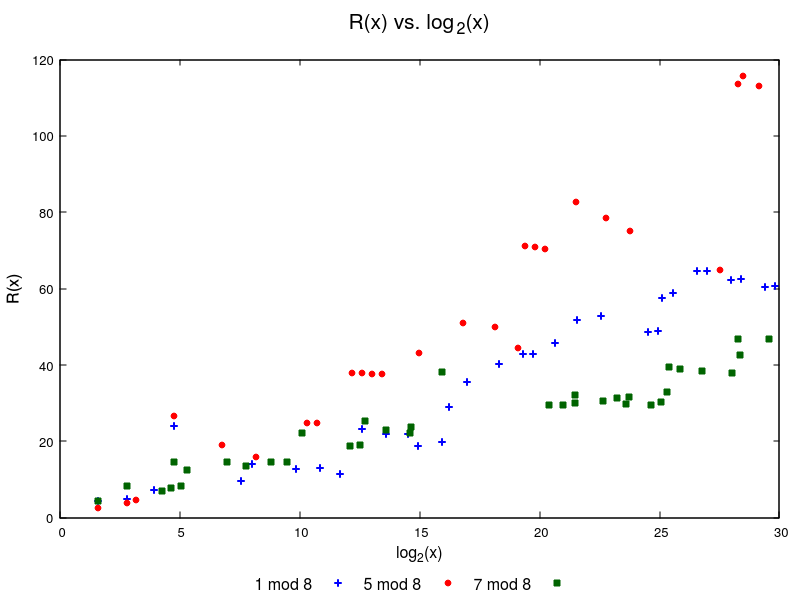
\includegraphics[scale=0.75]{ModAvoidanceAnalysisPics/R_vs_log.png}
    \caption{This graph visualizes how the $R$ values for $1 \Mod{8}$, $5 \Mod{8}$, and $7 \Mod{8}$ compare to each other. The log of the record holding numbers, or number of bits needed, is the x-axis, and the hardness measure $R$ as defined in section~\ref{subsec:rewritemeasuredefs} is the y-axis.}
    \label{fig:rvslog}
\end{figure}
However, it is clear that all three cases don't have the same slope of increase. $7 \Mod{8}$ has the most gradual growth of all three cases, followed by $1 \Mod{8}$ and $5 \Mod{8}$, which has not only the most growth, but the highest standard deviation of all three cases. These can be explained by the following observations:
\begin{itemize}
    \item Avoiding $7 \Mod{8}$ eliminates the growth of the $6 \rightarrow 7 \rightarrow 6$ cycle, meaning the numbers tend to get smaller and need less bits to encode as a rewrite string.
    \item Avoiding $5 \Mod{8}$ eliminates the decay of the 0 self-cycle, meaning numbers tend to grow more often than not, so the numbers here are larger.
    \item Avoiding $1 \Mod{8}$ is in between the other two cases, since both the 0 self-cycle of decay and the $6 \rightarrow 7 \rightarrow 6$ of growth can occur.
\end{itemize}
%This is all proof for showing how these rules correspond to the base 4 graph. I feel like this is unncessary for now, but I'll keep it in mind.
%We can actually expand our input strings to have two bits instead of 1, and with substitutions of certain rules, we can replace these two rules with 4 rules that results in an equivalent system. We also add a leading $x$ character, which means $x$ can be either $a$ or $b$.\footnote{$x$ could be any other character in the rewrite system except $d$, but none of these cases are interesting. If $x = c$, this system is nearly terminating, as this string corresponds to a number less than 8, which we know converges to 1. If $x$ is a ternary $e$, $f$, or $g$ character, then the $A$ and $B$ rules ensure we move the ternary character further left, so $x$ would turn into $a$ or $b$ as a result.} Here are the rules:
%\begin{align*}
%    D_1: xaad &\rightarrow xad &\text{$0\Mod{4}$}\\
%    D_2: xabd &\rightarrow xfad &\text{$1\Mod{4}$}\\
%    D_3: xbad &\rightarrow xbd &\text{$2\Mod{4}$}\\
%    D_4: xbbd &\rightarrow xgbd &\text{$3\Mod{4}$}
%\end{align*}
%These rules handle numbers based off of their last two bits, like the base 4 graph concerns the last 2 bits of numbers. Note that $D_1$ and $D_3$ in this new system are actually redundant rules. They could be replaced by the original $ad \rightarrow d$ rule and the system would function the same, but this example is just used to clearly show how the rewrite system ties to the graph. We do keep the odd rules in mind, as they will be important in simplifying the rewrite system down the road, particularly rule $D_4$. \par
%We now show how these rules correspond to the mod 4 graph. First, look at rules $D_1$ and $D_3$, the even rules. Both divide by 2, so an $a$ disappears. We look at the value for $x$ to determine what the new mod 4 value will be. For $D_1$, if $x$ is $a$, we end the string with $aad$, or $0 (\Mod{4})$, and we've hit the self loop of the graph, repeating rule $D_1$ for the next step. Else, if $x$ is $b$, we now have the string ending with $bad$, or $0 (\Mod{4})$, and apply rule $D_3$, also like in the graph. For $D_3$, in both cases, we end up with an odd number, because we end with a $b$, denoting a 1 bit, so if $x$ is $a$, we have $abd$, or $1 (\Mod{4})$, and if $x$ is $b$, we have $bbd$, or $3 (\Mod{4})$.\par
%The odd rules are trickier to explain, because the initial $bd \rightarrow gd$ rule, as discussed, actually computes $\frac{3x+1}{2}$. Hence, applying either of these rules actually results in a corresponding jump of two nodes. Since we've established the even nodes as having the correct transitions in the graphs, we can identify which node we go to given the transitions after applying rules $D_2$ and $D_4$. For $D_2$, if $x$ is $a$, we apply rule $A_2$, $af \rightarrow eb$, meaning our string ends with $bad$, so our next $D$ rule will be $D_3$. If $x$ is $b$, we apply $B_2$, $bf \rightarrow ga$, so our string ends with $aad$, and we apply $D_1$. This suggests that $D_2$ must transition to $0 (\Mod{4})$ because $0 (\Mod{4})$ can transition to rules $D_1$ or $D_3$, but not $2 (\Mod{4})$. This agrees with our graph. \par
%For $D_4$, if $x$ is $a$, then we apply rule $A_3$: $ag \rightarrow fa$. Our string ends with $abd$, so we're at $1 (\Mod{4})$, and apply rule $D_2$. Else, if $x$ is $b$, we apply rule $B_3$: $bg \rightarrow gb$, making our string end with $bbd$, and we apply rule $D_4$ once again. These paths correspond to coming from the $2 (\Mod{4})$ node, meaning $3 (\Mod{4})$ transitions to $2 (\Mod{4})$. Hence, this also agrees with the graph, and all of the $D$ rules in the new system agree with the graph. \par
%\subsection{Base 8 graph and rewrite tie together}
%Here are rewrite rules that correspond to this graph:
%These are now above.
%We omitted the $x$ this time, as we won't prove that they correspond to the graph. The approach is similar to what we had for base 4. Once again, the even rules are redundant, but the odd rules will be helpful in constructing a more efficient revised system. \par

\chapter{Conclusion} \label{sec:conclusion}
In this Thesis, we analyzed the Collatz Conjecture and simpler subproblems, and propose a hardness metric for determining the answers to these subproblems. We started by building a program that investigates Collatz Subproblems by running many $3x+1$ sequences for all odd numbers up to 1 billion, and seeing how many odd numbers occur in record breaking sequences that avoid the Collatz Subproblems. \par
We also investigated the Collatz SRS that Aaronson came up with in~\cite{HeuleAaronson} and that Heule tried to prove with Matrix Interpretation. Even though this methodology was not able to solve the Collatz Conjecture, we still think it has promise. We also built a simple program that ran the Collatz SRS and determine the hardness for subproblems, finding out that the hardness varies more than in the algebraic case.\par
As described in ~\cite{HeuleAaronson}, we believe this approach for trying to solve the Collatz Conjecture, as well as Collatz Subproblems, has merit and needs further investigation, so we hope to continue to do so in the future.




%%%%%%%%%%%%%%%%%%%%%%%%%%%%%%%%%%%%%%%%%%%%%%%%%%%%%%%%%%%%%%%%%%%%%%
% Appendix/Appendices                                                %
%%%%%%%%%%%%%%%%%%%%%%%%%%%%%%%%%%%%%%%%%%%%%%%%%%%%%%%%%%%%%%%%%%%%%%
%
% If you have only one appendix, use the command \appendix instead
% of \appendices.
% I MAY have an appendix later on with results.
%\appendices
%\index{Appendices@\emph{Appendices}}%

%\chapter{Lerma's Appendix}
\index{Appendix!Lerma's Appendix@\emph{Lerma's Appendix}}%
The source \LaTeX{} file for this document is no longer quoted in
its entirety in the output document. A \LaTeX{} file can 
include its own source by using the command
\cn{verbatiminput\{\cn{jobname}\}}.



%%%%%%%%%%%%%%%%%%%%%%%%%%%%%%%%%%%%%%%%%%%
\chapter{My Appendix \#2}
\index{Appendix!My Appendix \#2@\emph{My Appendix \#2}}%
\section{The First Section}
This is the first section.
This is the second appendix.

\section{The Second Section}
This is the second section of the second appendix.

\subsection{The First Subsection of the Second Section}
This is the first subsection of the second section of the second appendix.

\subsection{The Second Subsection of the Second Section}
This is the second subsection of the second section of the second appendix.

\subsubsection{The First Subsubsection of the Second Subsection of
		the Second Section}
This is the first subsubsection of the second subsection of the
second section of the second appendix.

\subsubsection{The Second Subsubsection of the Second Subsection
		of the Second Section}
This is the second subsubsection of the second subsection of the
second section of the second appendix.


%%%%%%%%%%%%%%%%%%%%%%%%%%%%%%%%%%%%%%%%%%%
\chapter{My Appendix \#3}
\index{Appendix!My Appendix \#3@\emph{My Appendix \#3}}%

\section{The First Section}
This is the first section.
This is the third appendix.

\section{The Second Section}
This is the second section of the third appendix.





%%%%%%%%%%%%%%%%%%%%%%%%%%%%%%%%%%%%%%%%%%%%%%%%%%%%%%%%%%%%%%%%%%%%%%
% Generate the bibliography.					     %
%%%%%%%%%%%%%%%%%%%%%%%%%%%%%%%%%%%%%%%%%%%%%%%%%%%%%%%%%%%%%%%%%%%%%%
%								     %
% NOTE: For master's theses and reports, NOTHING is permitted to     %
%	come between the bibliography and the vita. The command      %
%	to generate the index (if used) MUST be moved to before      %
%	this section.						     %
%								     %
\nocite{*}      % This command causes all items in the 		     %
                % bibliographic database to be added to 	     %
                % the bibliography, even if they are not 	     %
                % explicitly cited in the text. 		     %
		%						     %
\bibliographystyle{plain}  % Here the bibliography 		     %
\bibliography{bibliography}        % is inserted.			     %
\index{Bibliography@\emph{Bibliography}}%			     %
%%%%%%%%%%%%%%%%%%%%%%%%%%%%%%%%%%%%%%%%%%%%%%%%%%%%%%%%%%%%%%%%%%%%%%


%%%%%%%%%%%%%%%%%%%%%%%%%%%%%%%%%%%%%%%%%%%%%%%%%%%%%%%%%%%%%%%%%%%%%%
% Generate the index.						     %
%%%%%%%%%%%%%%%%%%%%%%%%%%%%%%%%%%%%%%%%%%%%%%%%%%%%%%%%%%%%%%%%%%%%%%
%								     %
% NOTE: For master's theses and reports, NOTHING is permitted to     %
%	come between the bibliography and the vita. This section     %
%	to generate the index (if used) MUST be moved to before      %
%	the bibliography section.				     %
%								     %
%\printindex%    % Include the index here. Comment out this line      %
%		% with a percent sign if you do not want an index.   %
%%%%%%%%%%%%%%%%%%%%%%%%%%%%%%%%%%%%%%%%%%%%%%%%%%%%%%%%%%%%%%%%%%%%%%


%%%%%%%%%%%%%%%%%%%%%%%%%%%%%%%%%%%%%%%%%%%%%%%%%%%%%%%%%%%%%%%%%%%%%%
% Vita page.							     %
%%%%%%%%%%%%%%%%%%%%%%%%%%%%%%%%%%%%%%%%%%%%%%%%%%%%%%%%%%%%%%%%%%%%%%

\begin{vita}
Matthew Alexander Denend was born in Spokane, Washington. He received the Bachelor of Science degree in Electrical Engineering, cum laude, from The University of Washington, Seattle, in 2012. He worked as a Packet Core Performance and Handset Engineer at T-Mobile in Bellevue, Washington for 3 years. He decided to pursue a Master of Science in Computer Science degree, and after he was accepted to The University of Texas at Austin in 2015, he left his job at T-Mobile to move to Austin, Texas and become a full-time student.
\end{vita}

\end{document}
